{\centering
\parbox{\textwidth}{%
  \raggedright{\itshape%

  You can't do inference without making assumption.\par\bigskip
  }
  \raggedleft\MakeUppercase{A Bayesian friend}\par%
}}

\chapter{Probabilistic modelling}\label{ch:02}

\begin{chapter_outline}

  The previous chapter established that modelling has played a major role in the progress of science and engineering.
  In this chapter, we argue that accounting for uncertainty is crucial for many, if not all, modelling tasks.
  \\
  This chapter is on \textit{probabilistic modelling} and shall answer the following questions:
  \begin{enumerate}
    \item What is a probabilistic model?
    \item How do we build a probabilistic model?
    \item How can we use a probabilistic model?
    \item What are the technical challenges considered in this thesis?
  \end{enumerate}
    For this purpose, we start by abstracting the concepts ruling probabilistic modelling and motivating the relevance of developing powerful tools in this context. We also present material to apprehend two classes of models relevant to this thesis, probabilistic graphical models and deep probabilistic models. Our discussion provides a high-level overview of these models and their different trade-offs.
% This chapter concerns the definition of unsupervised learning with a brief review of classical methods.
% Graphical models (in particular B-net are introduced here.)
% It continues with a review of deep generative modelling, with a discussion between explicit and implicit generative modelling.
% We introduce the concepts of GANs, Energy based models, VAEs, Normalizing Flows and diffusion models. With a note that VAEs and diffusions models
% are discussed in more details in further chapters.
\end{chapter_outline}

% \textcolor{red}{Clearly mention that deep generative models is a class of probabilistic model and so it is important to first clarify what are probabilistic models; why they are useful and why this is still q very qctive reserch area. (it might be simple to add this in the outline.)}

\section{Introduction}
The invention of computers enabled the automatisation of many tasks historically accomplished by humans. One key ingredient of this revolution is the ability to let computers reason - to make an informed judgment based on logical arguments and observations. The set of hypotheses on which this logic builds is a \textit{model}. Both humans and machines rely on reasoning to perform tasks. As an example, let us consider that we want to choose a bottle of wine at the restaurant. We first need some hypotheses, e.g., - What kind of wine do people like at the table? Red or white? Strong or delicate? - What is the budget? - What are we going to eat tonight? - What is the wine list? Etc. Provided this model, we can make an informed choice: remove the wines that are too expensive or would unpleased someone at the table, and \textit{wine not} pick one of the remaining that goes well with tonight's dinner? More seriously, a scientist needs a model of the earth and its atmosphere to explain climate change. Youtube considers your videos historical and a model that relates watched videos to recommendations to suggest videos. In these contexts and many others, the model plays a central part. We want good models, ones that lead to proper judgment. One that leads to the right wine, one that fits the climate over the last centuries, one that makes you click on one of the suggested videos.

Of course, the definition of a good model depends on its end application. However, certain classes of models are usually strictly better than others.
In particular, a model that embeds notions of uncertainty is more powerful than the fully deterministic version. It is because deterministic models do not faithfully represent phenomena that exhibit some forms of randomness inherent to our lives. Although it is unknown whether the laws that rule our reality are deterministic or stochastic, modelling requires simplifying assumptions inducing randomness. These assumptions often handle hidden factors that we cannot directly observe, noisy measurements or simplifying approximations. They are inherent in modelling a complex phenomenon, hence the induced stochasticity.

We thus need a language to express this stochasticity. The language of \textit{probability} is the one to make statements about uncertain events. It allows contrast between what is possible versus what is plausible. The distinction is essential as it will enable us to eventually make deterministic decisions by neglecting the most unlikely events and focusing on plausible events. An old bottle has a higher chance of being corked than a recent one. On the opposite, it might also taste better. We can use probability to express this fact and select a bottle to our taste with high probability.

\subsection{Probabilistic model}
A probabilistic model is a model that describes a phenomenon of interest in probabilistic terms. Practically, it defines a probability distribution between the set of variables considered valuable to describe the phenomenon (e.g., $X, Y, Z$). When it models the joint observations, the distribution can be the joint between all variables (e.g., $P(X, Y, Z)$). It can also be a conditional distribution  (e.g., $P(X \mid Y, Z)$) if we consider some of the variables known when using this model. We mostly limit our discussion to the former case for simplicity but with no loss of generality.

\begin{side_note}{Formalism}
  In this background, we will abstract the domain (discrete or continuous) of the random variables when possible. The term (conditional) probability distribution refers to the object $P$ that fully describes the stochastic behaviour of a random variable $X$ taking values in $\mathcal{X}$. When the domain $\mathcal{X}$ is discrete, $P$ corresponds to the probability function $P(X=\cdot): \mathcal{X} \rightarrow \left[0, 1 \right]$ that satisfies the three Kolmogorov's axioms. In the case of a continuous domain, we will narrow our discussion to real values $\mathcal{X} \triangleq \mathbb{R}^d$, where $d$ is the dimensionality of the random variable. In this context, the probability distribution is the density function $P(X=\cdot): \mathcal{X} \rightarrow \mathbb{R}_{+}$ which defines the probability that a realization $\bm{x}$ of $X$ lies in a sub-domain $\mathcal{A}$ as $\int_{\bm{x} \in \mathcal{A}} P(X=\bm{x}) \text{d} \bm{x}$. The probability functions implied by the density must also satisfy Kolmogorov's axioms. We will also clearly mention the domain of the random variable when it will matter for the discussion. Later in the thesis we focus on the continuous case and use a lowercase $p$ to denote the probability density function.
\end{side_note}
% For discrete variables, the mathematical object $P(X, Y, Z)$ is a probability and a density for continuous variables. In the following of this chapter, we will often use the symbol $P$ with no additional mention of the variable's type (discrete vs continuous) to generalise the discussion to both types.

One goal of building a probabilistic model, arguably the main one, is to perform \textit{inference}. That is to answer questions in the context of the models. These questions come in different flavours. What is the most likely value of $Y$ if we are to observe $X$? What is the conditional distribution of $Y$ in this case? Do we want to evaluate the value $P(Y \mid X)$ or just sample from it? For these purposes, the probabilistic models may have to handle different types of queries: \textit{marginalization, conditioning, sampling, and probability evaluation}.

Certain representations are appropriate for a subset of queries and not for others. For example, we can represent the discrete distribution between $X, Y, Z$ with a $3$D table where each entry stores the corresponding joint probability. The evaluation of the joint probability is very efficient with this representation. However, evaluating a conditional distribution requires going over each entry corresponding to the conditioning value and re-normalising the probabilities by their sum. Sampling becomes very inefficient as the number of entries in the table grows. And this number grows exponentially with the number of dimensions. Fortunately, there exist other representations that have different advantages and drawbacks. We will review those relevant to this thesis later in the chapter.

The following sections provide an overview of two main classes of probabilistic models, namely \textbf{Graphical models} and \textbf{Deep generative models}. As the name says, the former class aims for a graphical representation of the distribution. It allows us to understand modelling assumptions such as independence hypotheses quickly. The latter focuses on models whose internal representations use deep neural networks. These models are usually well suited for sampling. We will discuss the particularities of each class of models and will provide a thorough description of the main algorithms. We will also detail some algorithms to perform the different queries aforementioned on these models. \textcolor{red}{Say somewhere that all our contributions are on generative models, models that are efficient to sample from.}

In this manuscript, we will argue on multiple occasions that we shall not make a rigid distinction between graphical models and deep generative models as they are just different representations of the same mathematical object. Some deep generative models have a direct correspondence within the graphical family which enables abstract reasoning independent from the neural network architectures. However, for clarity, we will first introduce probabilistic graphical models. And then borrow the newly introduced notations and concepts to describe several deep generative modelling algorithms.


\begin{side_note}{Bayesian vs frequentist interpretation}
  Two interpretations of probabilities compete with each other. In the above discussion, we brought probabilities as a language to express our uncertainty about the truth of facts. We took the \textit{Bayesian} interpretation of probabilities. The reference to sir Bayes comes from the application of Bayes' rule to update our prior belief in the presence of new evidence. In this context, the prior is part of the model and affects its quality. The main drawback of the Bayesian interpretation is that it is sometimes hard to define the prior appropriately. The other view, referred to as \textit{frequentist}, interprets a probability as a frequency of events. With this perspective, probability does not quantify uncertainty; it expresses intrinsic randomness. Frequentists reject the notion of prior belief, which has pros and cons. In general, there is no interpretation better than the other. However, the Bayesian interpretation arguably provides solid explanations for popular algorithms in machine learning and is the one we will often implicitly use in our discussions. At the same time, we do not strictly reject the frequentist point of view. For example, we make many references to the maximum likelihood principle, which is fundamentally frequentist.
\end{side_note}
% Now contrast between discriminative versus descriptive models.
%
% Say that what differentiate models is the intrinsic distribution modeled but also in practice the exact way the distribution is expressed is important (reference to implicit versus explicit).

\subsection{Learning}
Before jumping into the description of different classes of models, we can keep our discussion general longer.
Until now, we have implicitly assumed the model was given to us. However, this is not realistic in many exciting settings. For example, how can I create an accurate model of my wine taste? Indeed, I cannot simply come up with a list ranking all world's wines. It might be too expensive to make and would not help me finish this dissertation. However, I could answer a long list of questions and then figure out a summary of my tastes for the principal characteristics of wine. The task of summarising my answers is learning - to build a compressed representation of observations (my answers). Afterwards, we can use this representation to perform an informed guess. This representation is a model, a simplified representation, of my wine taste. Learning is thus the task of instantiating a model from data.

In practice, we do not perform \textit{learning} without additional assumptions. Instead, we define a set of models among which we believe at least one would be a good representation of the phenomenon of interest. If we are Bayesians, we even add a probability that summarises whether or not we believe the model is good. We will come back to this later. For now, let us assume we do not have such a priori.

The class of possible models can be finite, e.g. the class contains two models - one for people who like red wine and white wine; the other for people who only like red wine. Compressing my taste into one of these models would go with a significant loss of information but might already be helpful in some settings. The class of models can be infinite, e.g. if parameterised by real values. For example, we can summarise wine taste by attributing an affinity score to each of the main features of wine.
\paragraph{Maximum likelihood estimation.}
A learning strategy is a set of rules that produce a model from data. When we only consider a finite number of models, a simple strategy exists. We test the predictive performance of each model and select the one that is the most consistent with our data. If the models describe the phenomenon with discrete events, we maximise the probability. If it considers a continuous set of events, we maximise the density. In the case where one of the models is \textit{correct} - it is the one that generates the data - this selection algorithm will eventually select the right model as the number of independently and identically distributed (iid) data points tends to $\infty$. This selection technique thus is said \textit{consistent}.

We can use a similar approach when the models are parameterized by a real vector $\bm{\theta}$. In this case, our goal is to estimate a good value for $\bm{\theta}$. One approach, denoted maximum likelihood estimation (MLE), is to select the model's parameter $\bm{\theta}$ that maximizes the  joint distribution (density or probability) of the data $\mathcal{D}$ provided its value. This quantity is called the likelihood function of the parameter $\bm{\theta}$, denoted $\mathcal{L}(\bm{\theta}) \triangleq P(\mathcal{D}\mid\bm{\theta})$. Hence the MLE estimator is formally defined as
\begin{align}
   \bm{\theta}_{\text{MLE}} = \argmax_{\theta} P(\mathcal{D}\mid\bm{\theta}). \label{eq:chap02:MLE}
\end{align}
In the presence of iid data, this estimator is consistent - provided a class of models that contains the `true` generative process, it eventually recovers the `true` model as the number of points tends to $\infty$. Formally, the consistency property is a convergence in probability of the estimator to the exact value and requires additional assumptions that ensure the model is identifiable and the likelihood function is well behaved (compactness and continuity to $\bm{\theta}$, and dominance).

The consistency of the MLE learning method makes it appealing. However, we must consider the central assumption very carefully! While ensuring that the model class contains the true generative process is ok in artificial settings. For real data, this assumption is almost a metaphysical question. The law of large numbers saves us if we only look at things on average and are provided with many data, but it does not apply to all modelling tasks. Sometimes, we know this assumption does not hold, but we would still like to learn a good model; the MLE principle does not say much. Even when we can be sure that the model class contains the correct model (e.g. we consider a parametric universal density approximator), we know nothing about the convergence speed. And this is without mentioning the optimisation procedure when there is no closed-form solution to \Cref{eq:chap02:MLE}.


\paragraph{Learning as inference.}
The strict delimitation between possible and impossible models is another limitation of the MLE approach. The model is either part of the class of models and is as likely as others to be the right one, or it is certainly irrelevant and is ignored. We can avoid the strict separation between possible and ignored models by reformulating learning. Instead of interpreting learning as model selection, we see learning as a particular inference task. We are thus back in a setting where the model is provided; however, it is fine as we can consider the model as a very generic description of the phenomenon. For example, the model can be a parametric function, exactly as when we define a class of models in the MLE approach. The distinction between learning as inference and MLE lies in our interpretation of the parameters. In the former, we consider the parameter $\bm \theta$ as part of the model rather than defining the class of models. While learning via MLE is usually associated with a frequentist interpretation of probability, learning as inference is Bayesian.

Let us consider the case where we want to learn a model that represents the conditional distribution $\argmax_y P(Y=y\mid\bm X=x)$ that I like a wine with features $\bm x \in \mathbb{R}^d$, where $y \in \mathbb{R}$ says if I like ($\rightarrow \infty$) or hate ($\rightarrow \infty$) a wine. We could consider a neural network that is parameterized by $\bm \theta$ and represents a parametric density function conditioned on a input $x$: $f(\cdot, \bm x;\bm \theta): \mathbb{R} \times \mathbb{R}^{d} \times \mathbb{R}^{\lvert\bm \theta\rvert} \rightarrow \mathbb{R}^+$.
Learning aims at summarising the information in the data to perform a task of interest, here to predict $P(Y \mid X, \mathcal{D})$.
If we state that $f$ represents the conditional distribution $P(Y\mid X, \bm \theta)$, this gives
\begin{align}
  P(Y=y\mid X=\bm x, \mathcal{D}) &= \int P(Y=y\mid X=\bm x, \bm \theta) P(\bm \theta \mid \mathcal{D}) \text{d}\theta\\
  &=\int f(y, \bm x;\bm \theta) p(\bm \theta \mid  \mathcal{D}) \text{d}\theta.
\end{align}
We notice that the data are only used through the posterior distribution of the parameters $\bm \theta$. The posterior summarises our belief about which models best describe the phenomenon of interest in light of the data observed and our initial belief. The goal of learning is thus to compute $P(\bm \theta \mid \mathcal{D})$, which is an inference task. \textcolor{red}{how shall I mention functional form, I am not sure about the right vocabulary. We replace $P(\bm \theta)$ by $P(f)$} - mention kernel methods that naturally work in a function space.  very general hypothesis space might be the class of smooth functions $\mathbb{C}_\infty$ from $\mathbb{R}^d$ to $\mathbb{R}$.

It is often cumbersome to keep track of the complete posterior distribution in practice. We can avoid this by selecting the maximum a posteriori (MAP) sub-model. In the case of a parametric model this means freezing the parameter $\bm \theta$ to their most plausible value $\bm \theta_{MAP} = \argmax_{\bm \theta} P(\bm \theta \mid \mathcal{D})$. Learning as inference strictly generalises the MLE principle to settings where the prior knowledge is more subtle than possible or impossible. When we consider a non-informative prior, the method is equivalent to the MLE. And when we do have a good prior, this strategy will naturally reduce the importance of bad model instantiation and mostly rely on the instantiations that were plausible and described well the data. Moreover, this approach is consistent and eventually selects the `right` instantiation.

Learning as inference is sometimes criticised by practitioners who do not like the concept of attributing plausibility to the different instantiations of the model. However, this criticism is empty from my point of view. The superiority of this approach relies on the obligation to explicit the modelling assumptions and the plausibility associated with each learnable component of the model. It forces us to acknowledge that learning a model is a subjective task. As an example, Occam's razor says that we should always favour the simplest among potential explanations. The Bayesian approach naturally handles Occam's razor by attributing higher plausibility to simpler model instantiations. This is not true for the MLE approach, which requires adding an ad-hoc rule or regularisation objective to the optimisation problem.

% Say that the joint distribution defined by the probabilistic is sometimes learned conditionaly to an input x, without caring about modelling the distribution over x. This is what is called supervised learning. Usually contrasted with unsupervised learning that looks at an uncondiotnal joint distribution. This distrinction is orthogonal to the one of probabilistic modelling.
%
% Say about the correspondance between what seems ``deterministic'' supervised machine learning and that it always correponds to strong assumptions on the form of the distribution.
\paragraph{Machine learning = probabilistic modeling.}
\begin{figure}
  \centering
  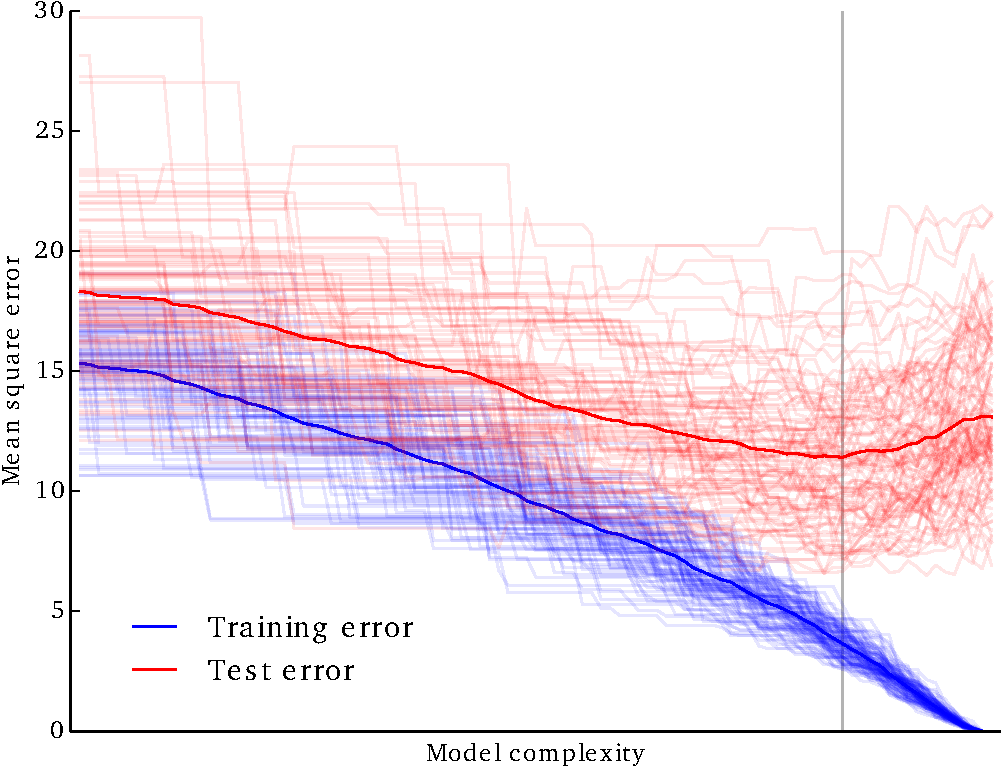
\includegraphics[width=.5\textwidth]{figures/chapter02/ch2_train_test_error.pdf}
  \caption{This plot is taken from \citet{louppe2014understanding}. It shows the necessary trade-off between the model's complexity and generalisation performance. As the model gets too complex, it starts overfitting the training data, decreasing test performance.}
  \label{fig:ch02:learning_curves}
\end{figure}
The attentive reader will notice that machine learning (ML) was only mentioned once until now, when discussing the bayesian and frequentist interpretations of probability.
This may sound surprising as this thesis aims to build bridges between ML algorithms and the classical modelling approach. We did this on purpose as the distinction between classical modelling (as performed by domain experts, e.g. in science or engineering) and ML is often irrelevant. We have described probabilistic modelling in generic terms that are valid for both approaches. Whether the class of models is small, made of well-understood pieces, or a huge neural network does not matter when describing the key steps to building and using a model. Even a model designed with domain knowledge usually has degrees of freedom to adapt the model to contexts. At the same time, it is not because we do deep learning with much data that we must forget that learning relies on assumptions.

It is interesting to use a bayesian interpretation of the learning algorithm inductive bias to explain its generalisation property. Taking the bayesian prospect allows drawing many connections between classical modelling and ML. One aspect of classical modelling is considering small classes of models that usually contain simple models. This is well-aligned with Occam's razor and often leads to good models when the studied process is well understood. Machine learning is often applied to problems for which classical modelling fails because we cannot create a simplified representation of the phenomenon by ourselves. This does not mean ML's job is to learn a complex model of the phenomenon, quite the opposite. As depicted in \Cref{fig:ch02:learning_curves}, an ML model achieves its best predictive performance by balancing the model's complexity and goodness of fit. This behaviour is arguably observed with any ML algorithm, although defining a model's complexity is not always straightforward. A standard method to control the complexity of an ML model is to split the data into a training, a validation and a test set. The validation set is used to find the hyperparameters of the learning algorithm that lead to a trained model that generalises well, that is, a model that has a good balance between faithfulness and complexity. We then use these hyperparameters to learn a new model with both train and validation sets and use the test set to assess whether generalisation happens. % access an unbiased estimation of the model's complexity.

Machine learning algorithms are sometimes described in deterministic terms. For example, a classical ML task is to predict a real value $y$ provided a set of features $\bm x$. At first glance, we might have trouble interpreting this in the probabilistic framework, limiting the scope of our previous discussion to a subset of ML algorithms. This is not the case as a deterministic model always has correspondence in the probabilistic framework. The corresponding class of models makes strict assumptions about the distribution's shape instead of using data to learn it.

For example, fitting a regression model with mean squared error is equivalent to considering that $P(Y\mid X)$ is a gaussian distribution with a fixed variance. Similarly, mean absolute error corresponds to a Laplace distribution. The duality between the deterministic and the probabilistic interpretations goes further as we can also interpret the learning algorithm as the application of MLE or MAP principles. % when additional regularization is used to explicitly control the model's complexity.

Another important aspect of modelling is to select the appropriate class of models. This choice highly depends on the final application as different applications may require performing distinct types of queries on the model. In addition, the learning scenario may also differ and impacts the suitability of different models. As we will see soon, different classes sometimes correspond to very different inference algorithms. Some models represent the distribution of interest as a sampling procedure, while others provide access to the probability density function (pdf). If our goal is to generate samples, we might prefer the former models, although we could also use Markov chain Monte Carlo to sample from a pdf. The following sections aim to shed light on some powerful classes of probabilistic models that exhibit different advantages and shortcomings.

%
% Things to mention:
% - Why we need train/valid/test (also for probabilistic); Provide the complexity plot.
% - Why using MSE or L1 error is equivalent to maximizing likelihood and adding a penalty to the parameters is equivalent to MAP.
% - How do we chose the learning algorithms/class of models? This a function of what we want to achieve with the model.

\section{Probabilistic graphical models}

As the saying goes, a picture is worth a thousand words. It is why we start our journey in the probabilistic-model lands by revisiting probabilistic graphical models (PGMs). Our trip will pass by Bayesian network, and will make a small detour by Markov networks, hoping to not leave the interested reader on the side of the road. As their name hints, PGMs have in common their reliance on graphical representation. We will observe that directed and undirected graphs have many relevant properties to represent modeling assumptions such as known (in)dependence. These representations lead to specialized inference and learning algorithms which will be discussed after.

The introduction of an undirected representation of the distribution of interacting particles in 1902 by Gibbs might be one of the first PGM. We can also attribute one of the first directed PGM to Sewal Wright who studied genetics back in the 1920's. The statistics community only started to ackowledge the graphical framework in 1960's. And it is even later, in in the late 80's, that PGMs started to creep in the field of artificial intelligence (AI) with the seminal works of Judea Pearl and his colleague that provided algorithms to take advantage of Bayesian networks, a class of directed PGMs. Since then, the graphical representation has been recognized as a powerful tool by many communities. It has achieved great successes such as in \textcolor{red}{cite cool applications}. Recently, causality, which is deeply rooted on Bayesian networks has arguably become one of the hot topic in ML and might be part of the greatest next successes in AI. \textcolor{red}{add citations}.

Many great resources on PGMs exist and our goal is not to compete with them. We provide sufficient materials to get the reader interested and understand the main advantages and limitations of standard algorithms. This provides a common ground between the reader and the author to motivate the connections with deep generative models and improvements to classical PGMs we have broughts in the scope of this thesis. We invite the reader interested by additional details to check \citet{koller_probabilistic_2009}, the main reference used to guide this introduction to PGMs.

\subsection{The curses of dimensionality}
% \textcolor{red}{add a figure that shows how the distance between two random points grows as the number of dimension grows.}
\paragraph{Learning is hard.} We consider a bunch of unfair coins $\bm{x} = \left[x_1, \dots, x_d \right]$. Given a dataset of simulatenuous throws $\mathcal{D} = \{\bm{x}_i\}_{i=1}^N$ , we want to learn a probabilistic model $P(X=\bm{x})$. A natural approach is to represent the joint probability as a $d$-dimensional array with an entry for each possible realization. In this context, learning corresponds to filling the $2^d$ values in the table. We can reduce this number by factorizing the distribution as
$$P(\bm{x}) = P(x_1)\Pi_{i=2}^d P(x_i\mid x_{<i}),$$ and by acknowledging that the (conditional) probabilities of a tail and a head sum up to $1$. Unfortunately we do not gain much as the number of entries in the table still grows exponentially ($\sum_{i=1}^d 2^{i-1} = 2^{d-1} - 1$) and learning still quickly gets very dificult with the number of dimensions. This phenomenon is broadly refereed as a \textit{curse of dimensionality} and also hits continuous variables. However this is just a recall to the reality as we always need assumptions to create models - good news is we can fight the curse of dimensionality with modelling assumptions. For example, it is reasonable to assume the coins independent, the joint distribution is then factorized into $d$ terms: $ P(\bm{x}) = \Pi_{i=1}^d P(x_i)$. For continuous variables smoothness and constraints on the possible types of interactions between variables may allow us to achieve modelling results that challenge the curse of dimensionality. We will see soon strategies to express different modelling assumptions.
% - If we do not restrain the hypothesis space or bias the learning in some sense the curse of dimensionality kills us. -> Learning is hard.

\paragraph{Sampling is hard.} We want to sample realisations provided the joint distribution $p(X=\bm x)$. To this end, we may use approximate sampling schemes (e.g., MCMC, or importance sampling) that rely on a proposal distribution (e.g., a normal distribution) and an acceptance/rejection strategy. As the number of dimension increases the gap between the proposal distribution and the one of interest will naturally grows, and the acceptance rate will collapse. This means we need to understand some modelling assumptions in order to develop efficient sampling strategy. We will see later how rewarding is the joined development of the model class and the sampling strategy.

\paragraph{Interpreting is hard.} The complexity of a model naturally grows with the number of variables we consider. Clearly, humans are not able to apprehend correctly more than a few dimensions. If our goal is to understand how different modelling assumptions impact the model it may be important to use specific framework for this. We will see that graphical models offer a nice balance between expressivity and interpretability and

\subsection{Directed graphical models - Bayesian networks}
If we do not make assumptions, probabilistic modelling becomes hopeless as the dimensionality grows for the reasons mentioned before. We now review one of the most popular strategies to fight the intractability of PGMs in high dimensions, Bayesian networks (BN). BNs are a class of models that enables independence to enter the list of modelling assumptions. As we have seen, representing $d$ simultaneous coins tosses requires the specification of at least $2^{d-1} - 1$ numbers. This number drops to $d$ if we consider all the variables independent. Indeed, it is reasonable to assume that the realisation of one coin toss does not help predict the outcome for another coin. Hence, the best model should be part of the subclass of models considered. BNs define a subclass of models with (conditional) independencies, allowing them to represent distributions more compactly. The term Bayesian can be attributed to the Bayes' rule, which factorises a joint distribution into compact factors.

\subsubsection{Bayesian networks}
\begin{figure}
    \centering
    \begin{subfigure}{.45\textwidth}
        \centering
        \begin{tikzpicture}[
          node distance=.7cm and 1.cm,
          var_x/.style={draw, circle, text width=.4cm, align=center}
        ]
            \node[var_x] (x1) {$X_1$};
            \node[var_x, right=of x1] (x2) {$X_2$};
            \node[var_x, below=of x1] (x3) {$X_3$};
            \node[var_x, right=of x3] (x4) {$X_4$};
            \path (x1) edge[-latex] (x2);
            \path (x1) edge[-latex] (x3);
            \path (x1) edge[-latex] (x4);
            \path (x2) edge[-latex] (x3);
            \path (x2) edge[-latex] (x4);
            \path (x3) edge[-latex] (x4);
            %\node (b) at (1,-3) {(\textbf{b})};
        \end{tikzpicture}
        \caption{}\label{fig:BN-fig-a}
    \end{subfigure}~\hspace{-4.8em}
    \begin{subfigure}{.45\textwidth}
    \centering
        \begin{tikzpicture}[
          node distance=.7cm and 1.cm,
          var_x/.style={draw, circle, text width=.4cm, align=center}
        ]
            \node[var_x] (x1) {$X_1$};
            \node[var_x, right=of x1] (x2) {$X_2$};
            \node[var_x, below=of x1] (x3) {$X_3$};
            \node[var_x, right=of x3] (x4) {$X_4$};
            %\node (a) at (1,-3) {(\textbf{a})};
            \path (x1) edge[-latex] (x3);
            \path (x1) edge[-latex] (x4);
            \path (x2) edge[-latex] (x3);
            \path (x2) edge[-latex] (x4);
        \end{tikzpicture}
        \caption{}\label{fig:BN-fig-b}
    \end{subfigure}
    \caption{Two Bayesian networks of a $4$D variable. (\textbf{a}) No independence. (\textbf{b}) A couple of independence, hence a reduced number of edges and of parameters.} \label{fig:BN-fig}
\end{figure}

A Bayesian network is a directed acyclic graph (DAG) that represents independence assumptions between the components of a random vector. Formally, let $X = \left[X_1, \hdots, X_d\right]^T$ be a random vector taking values $X \in \mathcal{X}_1 \times \dots \times \mathcal{X}_d$ distributed under $P_{X}$. A BN for $X$ is a directed acyclic graph with one vertex for each random variable $X_i$ of $X$. In this network, the absence of edges models conditional independence between groups of components through the concept of d-separation~\citep{geiger_d-separation_1990}. A BN is a valid representation of a random vector $X$ iff its probability distribution (continuous or discrete) factorizes as
\begin{align}
    P_{X}(X) = \prod^d_{i=1}P(X_i\mid \mathcal{P}_i),\label{eq:BN-fact}
\end{align}
where  $\mathcal{P}_i = \{X_j: A_{i,j} = 1 \}$ denotes the set of parents of the vertex $i$ and $A \in \{0, 1\}^{d\times d}$ is the adjacency matrix of the BN. A BN, together with the related conditional probability distributions, is a PGM. For simplicity, we will use the term BN to refer to this couple and explicitly mention the terms topology or structure when talking about the BN's structure.

\figref{fig:BN-fig} is a valid BN for any distribution over $X$ because it does not state any independence and leads to a factorisation that corresponds to the chain rule. However, in practice, we seek a sparse and valid BN which models most of the independence between the components of $X$, leading to an efficient factorisation of the modelled probability distribution. It is worth noting that making hypotheses on the graph structure is equivalent to assuming certain conditional independence between some of the vector's components.

Understanding the independence assumptions underlying a DAG is key to appreciating BNs. For this purpose, d-separation describes rules to check if conditional independence holds in all distributions that factorise over a DAG. This algorithm is described in \Cref{alg:d-separation} and allows checking whether the topology is well suited to model a phenomenon of interest. In addition, it also enables characterising all (conditional) independencies that follow from a set of distinct independence assumptions. D-separation is \textit{sound}, it only detects existing independence. However, it is not \textit{complete} as it misses independence assumptions hidden in the parameterisation of conditional distributions. For example, the BN in \Cref{fig:BN-fig-a} can model any joint distribution for $X$; applying d-separation to this graph would reject all independence, even though the distribution modelled could contain independence.

\begin{algorithm}
\caption{D-separation.}\label{alg:d-separation}
  \begin{algorithmic}
    \Function{IsIndependent}{$X$, $Y$, $Z$, $G$}
      \State \Comment{\small Return True iif $X \indep Y \mid Z$ is modelled by the Bayesian network with topology $G$.}
      \For{$N \in Z$}
        \State $P \gets \text{Parents}(Z)$ \Comment{Returns \textbf{directed} parents (v-structure if more than one)}
        \For{$P_i \neq P_j \in P$}
          \State $G \gets \Call{AddUndirectedEdge}{P_i, P_j, G}$
        \EndFor
        \State $G \gets \Call{RemoveNode}{N, G}$
      \EndFor
      \State \Return{\Call{IsNotReachable}{$X$, $Y$, $G$}}
    \EndFunction
   \end{algorithmic}
\end{algorithm}

\subsubsection{Parameterization}
The value of BNs is to reduce the description of a joint distribution to topology and a batch of $1$D conditional distributions. The topology is often prescribed by domain knowledge, while learning the conditional distributions from data is common. As mentioned earlier, learning aims at selecting (or weighting) within a class of models. A natural way to define a model class is to use parameters to describe the free parts of the model. For BNs, the free parts are usually only the conditional distributions as parameterising distributions is more straightforward and leads to simpler optimisation problems than graph structures. For discrete variables, we use categorical distributions, and each conditioning factor corresponds to distinct parameter values. Continuous variables offer many alternative parameterisations, e.g. the exponential family where parameters are a linear function of the conditioning factors. Gaussians with linear interactions are arguably one of the most popular parameterisations. These models, dubbed Gaussian Bayesian networks, were historically the only ones with an efficient training algorithm as they correspond to multivariate Gaussian distributions \citep{wermuth1980linear} for which closed-form MLE exists. In \Cref{ch:06}, we introduce normalizing flows as a more expressive parameterisation and use stochastic gradient descent to approach the MLE.
\subsubsection{Inference}
Inference is arguably the most elementary task we may perform provided a model. Here we focus on the generic the conditional probability query $P(Y\mid E=e)$, where $Y$ denotes a subset of the model's variable and $e$ is the value of another subset $E$ of the variables, the remaining variables $M = \{X_i: X_i \notin Y \cup E \}$ are marginalized out. For example, we might be interested in evaluating $P(X_1\mid X_3=x_3, X_4=x_4)$ in \Cref{fig:BN-fig}.

As mentioned earlier, inference gets more complicated when the number of variables increases. However, BN adds structure to this problem by making some of the independencies explicit. While inference in BN stays NP-hard in the worst case, there exist algorithms able to exploit the structure for most inference tasks efficiently. For example, Pearl's message-passing algorithm is an efficient exact inference algorithm that works only on polytrees, a subclass of BNs that only have uniparental nodes. Variable elimination (VE) is another popular algorithm that works on all discrete BNs and reduces the complexity of inference to the width (maximum distance between two nodes) of the graph. \citet{sanner2012symbolic} adapts VE to continuous variables with a symbolic version of VE. However, VE performs marginalisation and distribution products, which are not straightforward operations in the continuous setting.

\paragraph{Inference as sampling.}
The case of continuous variables motivates us to formulate inference differently. We look for formulations that do not explicitly mention marginalisation or product of densities. A natural solution is to replace exact inference with conditional sampling from $P(Y\mid E=e)$. Let us notice that we can sample from the joint distribution, hence from any marginal distribution, by traversing the graph from parents to children. This method is known as \textit{ancestor sampling}. At each node, we sample conditionally on the parents' value and eventually obtain a value for all nodes that is a valid sample from the joint distribution.

Ancestor sampling assumes that we have a procedure to generate samples for each factor $P(X_i\mid \mathcal{P}_i)$ which is usually straightforward. For example, provided the corresponding cumulative distribution function $F(\cdot;\mathcal{P}_i): \mathcal{X}_i \rightarrow \left[0, 1 \right]$ and a uniform random variable $U$ in $\left[0, 1\right]$, $x_i=F^{-1}(u;\mathcal{P}_i)$ follows $P(X_i\mid \mathcal{P}_i)$. This method is known as \textit{inversion sampling}. \textit{Rejection sampling} (RS) is an alternative strategy when we can only evaluate the joint distribution. The idea is to sample $z \in \mathcal{X}_i$ from a proposal distribution $P_z$, then accept the sample if $u< \frac{p_{x_i}(z)}{K P_z(z)} $ where $K$ is chosen such that $ K P_y(x_i) \geq P_{x_i}(x_i) \quad \forall x_i \in \mathcal{X}_i$.

RS works also when the joint distribution is only known up to a normalizing factor but becomes inneficient as the number of dimension grows. Another limitation appears if we want to condition on a subset of the sampled variables as it would reject all samples almost certainly in the continuous setting. It is also very inneficient for discrete BNs. A solution is to freeze the conditioning factors $E$ to their value $e$ and to notice that sampling from $P(Y\mid E=e)$ is equivalent to sampling from $P(Y, M\mid E=e) = \frac{P(Y, M, E=e)}{P(E=e)}$ and ignoring $M$. Such that \Cref{eq:BN-fact} provides the unormalized value of $P(Y, M\mid E=e)$. Then we can sample values $(y_1, m_1), \dots, (y_k, m_k)$ via ancestor sampling, and keep track of the corresponding weight $P(Y, M, E=e)$. We can use these weighted samples to efficiently approximate an expected value over the posterior distribution as
$$ \mathbb{E}_{P(Y\mid E=e)}\left[f(y)\right] \approx \frac{\sum_{i=1}^k f(y_i) P(Y=y_i, M=m_i, E=e)}{\sum_{i=1}^k P(Y=y_i, M=m_i, E=e) }.$$ For discrete variables this provides an approximate alternative to VE with $$P(Y=y\mid E=e) \approx \frac{\sum_{i=1}^k f(y_i) P(Y=\bm{1}\{y_i = y\}, M=m_i, E=e)}{\sum_{i=1}^k P(Y=y_i, M=m_i, E=e)}. $$ This method is known as \textit{likelihood weighting} and is a special case of \textit{importance sampling} when the proposal distribution is ancestor sampling. We can convince ourselves that likelihood weighting prefers when the conditioning factors are located at the root of the BN.

Although importance sampling uses samples more efficiently, it does not provide samples from the posterior distribution. Markov Chain Monte Carlo (MCMC) is a family of algorithms that describes asymptotically correct sampling procedure that only requires access to an unnormalised density function. These algorithms run a Markov chain whose stationary distribution follows the given density. The difference between MCMC algorithms lies in the transition probability $P(y^k\mid y^{k-1})$. Many instances exist, such as Metropolis-Hastings MCMC, Hamiltonian MCMC, slice sampling, etc. Gibbs sampling is an instance that aims to exploit the BN structure in the transition probability. Let us suppose that $M = \phi$, then at each transition step we only update one component $x_i$ of $y^k$, the transition probability updates $X_i$ from the posterior $P(X_i\mid x_{-i}^{k-1})$ where $x_{-i}^{k-1}$ contains the values of the evidence $E$ and the previous state $y^{k-1}$ except the $i^{\text{th}}$ component. This reasonably assumes that we can sample from the $1$D posterior efficiently.

% \textcolor{red}{Mention that we do not pretend to be complete as there exist many many algorithms and we only focus on generic algorihm that showcase some of the classical issuing when sampling from these models. I have to help the reader to understand better why he it is important that he reads this sections. For the one about sampling it shows that inference is really hard but adding strucure helps producing specialized algorithms. For the inference as optimization it must mainly motivates to create parametric models that are efficiently trainable. Also mention that although we try to keep the discussion generic, our interest is really for continuous variables in this thesis. Find a place to mention the Expectation–maximization algorithm.}

\paragraph{Inference as optimization.}
We now introduce variational inference (VI) as an alternative to sampling strategies. Variational inference formulates inference as an optimisation problem in which we look for a distribution $Q(Y)$ that is as close as possible to the posterior of interest $P(Y\mid E=e)$. For this purpose, we consider a parametric family of distributions $Q_\theta(Y)$, such as a BN with a prescribed structure but parametric distributions. Our goal is to optimise for the best set of parameters $\theta^\star$:
\begin{align}
  \theta^\star = \argmin_\theta \mathbb{D}\left[Q_\theta(Y)\Vert P(Y\mid E=e) \right], \label{eq:obj_VI}
\end{align}
where is an appropriate divergence between distributions. For the rest of this discussion, let us fix $\mathbb{D}$ to the Kullback-Leibler ($\mathbb{KL}$) divergence which is an appropriate choice as it is only minimized when $Q = P$. As of now, we also restrain our discussion to the case of continuous variables.

Solving $\label{eq:obj_VI}$ is possible if we have a parametric family of distributions for which density evaluation and sampling are differentiable functions of the parameters. Normalizing flows define such a family and will be described in the next section, but it could also be another BN. Let us denote by $Q_\theta$ the probability density function and the procedure to generate samples as $$ y := f_\theta(z) \quad\text{where}\quad z\sim \mathcal{N}(0, I),$$
where $\mathcal{N}(0, I)$ denotes a normal distribution.
In this ideal case, the optimization problem becomes:
\begin{align}
  \theta^\star &= \argmin_\theta \mathbb{KL}\left[Q_\theta(Y)\Vert P(Y\mid E=e) \right]\\ \label{eq:VI_optim}
  &= \argmin_\theta \mathbb{KL}\left[Q_\theta(Y)\Vert P(Y, E=e) \right] + \mathbb{E}_{\bm y}\left[\log P(E=e)\right]\\
  &= \argmin_\theta \mathbb{E}_{z}\left[ \log \frac{Q_\theta(f_\theta(z))}{P(f_\theta(z), E=e)} \right].
\end{align}
We can optimise the equation with stochastic gradient descent (SGD) by approximating the objective function with Monte Carlo samples at each gradient step.

However, evaluating $P(f_\theta(z), E=e)$ in the last equation is not always possible (e.g. the variables in $M$ have at least one child). In this context, we may create an approximation $Q_{\theta^\star}(Y, M\mid E=e)$ of $P(Y, M\mid E=e)$ instead. We can then generate samples from the joint and thus from the marginal $P(Y\mid E=e)$. If we need to evaluate the approximate $Q_{\theta^\star}(Y\mid E=e) := \int Q_{\theta^\star}(Y, M\mid E=e) \text{d}M$, we can find a surrogate model $\tilde Q_\psi$ by solving the following optimization problem:
\begin{align}
  \psi^\star &= \argmin_\psi \mathbb{KL}\left[Q_{\theta^\star}(Y, M\mid E=e)\Vert \tilde Q_\psi(Y) \right]. \label{eq:approx_posterior}
\end{align}
We can also optimize this equation with SGD and Monte Carlo samples as it only requires to sample from and evaluate $Q_{\theta^\star}(Y, M\mid E=e)$, and to evaluate $Q_\psi(Y)$. We can convince ourselves that the solution to \Cref{eq:approx_posterior} is $Q_{\theta^\star}(Y\mid E=e)$,
\begin{align}
  &\min_Q \mathbb{KL}\left[P(Y, M)\Vert Q(Y) \right]\\
  &=\min_Q \mathbb{E}_{P(Y) P(M\mid Y)}\left[\log P(Y) + \log P(M\mid Y) - \log Q(Y)\right]\\
  &=\min_Q \mathbb{E}_{P(Y) P(M\mid Y)}\left[\log P(Y) - \log Q(Y)\right]\\
  &= \min_Q \mathbb{E}_{P(Y)}\left[\log P(Y) - \log Q(Y)\right]\\
  &= \min_Q \mathbb{KL}\left[P(Y)\Vert Q \right].
\end{align}

VI requires a parametric distribution differentiable to sampling and density evaluation. The family of distributions must contain instances close to the true posterior to achieve good results. In addition, solving the optimisation can be complicated even if provided with a parametric universal density approximator. However, VI is preferable to sampling strategies for multiple reasons. It eventually becomes faster than sampling as \ref{eq:obj_VI} returns a model from which we can generate as many samples as wanted. This approach also automatically provides a surrogate of the posterior density. Finally, we can apply this approach to learning a parametric posterior distribution that approximates $P(Y\mid E=e)$ for any value of $e$.

Another interesting application of VI is for estimating a bound on the log-marginal $\log P(E)$ of the larger model $P(Y, E)$. We can directly derive from \Cref{eq:VI_optim}:
\begin{align}
  \mathbb{KL}\left[Q_\theta(Y)\Vert P(Y\mid E=e)\right] &\geq 0\\
  \mathbb{KL}\left[Q_\theta(Y)\Vert P(Y, E=e) \right] + \mathbb{E}_{y}\left[\log P(E=e)\right] &\geq 0\\
  \mathbb{E}_{\bm y \sim Q_\theta(Y=\bm{y})}\left[ \log \frac{P(E=e\mid Y=\bm{y}) P(Y=\bm{y})}{Q_\theta(Y=\bm{y})} \right] &\leq \log P(E=e)\\
  \underbrace{\mathbb{E}_{\bm y \sim Q_\theta(Y=\bm{y})}\left[ \log P(E=e\mid Y=\bm{y})\right] - \mathbb{KL}\left[Q_\theta(Y)\Vert P(Y)\right]}_{\operatorname{ELBO}} &\geq \log P(E=e) \label{eq:elbo}
\end{align}
This estimated lower bound on the evidence ($\operatorname{ELBO}$) is useful to approximate the log-likelihood of a parametric model $P_{\bm \psi}(E)$ defined as the marginal of a larger model $P_{\bm \psi}(Y, E)$.
We will see later that this the main technique for learning deep probabilistic models that formulates the generative process as a stochastic map from latent variables to observations.
% \textcolor{red}{Discuss the case of exact inference in continuous is maybe hopeless.}
\subsubsection{Learning}
We have just seen that inference can be formulated as learning a probabilistic model. We now describe strategies to learn the parameters of a BN.
A BN combines a graph $G \in \mathcal{G}$, where $\mathcal{G}$ denotes the set of DAGs, and the corresponding conditional distributions $f: \{P(X_i\mid \mathcal{P}_i)\}_{i=1}^d$ to model a joint distribution. Ideally, we would like to adapt both $G$ and $f \in \mathcal{F}$, where $\mathcal{F}$ is the set of considered conditional distributions (e.g. encoded by some parameters), to the learning dataset $\mathcal{D}=\{X^i\}_{i=1}^N$.

Assuming iid data, we can express the learning task as a generic optimisation problem:
\begin{align}
  B^\star  = \argmax_{B\in\mathcal{B}} \sum_{i=1}^N \log P_B(X^i) - R(B), \label{eq:learn_BN}
\end{align}
where $\mathcal{B} = \mathcal{G} \times \mathcal{F}$ denotes the set of possible BNs (assuming the right number of variables). $R(\cdot): \mathcal{G} \times \mathcal{F} \rightarrow \mathbb{R}$ is a regularisation term which can be interpreted as the prior over plausible BNs, it is a constant value if we do MLE. We insist on the importance of $R(B)$ for obtaining a good model. For example, we look for structures that are as sparse as possible although BNs with complete DAGs are strictly more expressive than sparser ones. In general, we aim for BN structures that reflect the indepence modeled.

The formulation in \ref{eq:learn_BN} does not say much about concrete strategies to fit the parameters of a BN. In practice, we often separate structure learning from distribution fitting. Structure learning is a combinatorial problem, whereas fitting the parameters of conditional distributions is a continuous optimisation problem; solving both issues jointly is an open problem. In \Cref{ch:06}, we will see one strategy to formulate the combinatorial problem into a continuous one; these are advanced concepts beyond this background's scope. Now, we focus on the two sub-problems independently.

\paragraph{Distribution learning.}
We suppose a prescribed topology and only focus on learning the best factors in \eqref{eq:BN-fact}. For this purpose we can parameterize the factors with a vector $\bm \theta$ and update \eqref{eq:learn_BN} into
\begin{align}
  {\bm \theta}^\star  = \argmax_{\bm \theta} \sum_{i=1}^N \log \prod^d_{j=1}P_{\bm \theta}(X_j^i\mid \mathcal{P}_j) - \log \pi(\bm \theta).
 \label{eq:learn_factors}
\end{align}
The choice of the parameterisation and the prior $\pi$ are crucial to finding a good model when $N$ is finite. Although parametric universal density approximators exist, such as normalizing flows, learning the parameters of these functions can be challenging when the dataset is small or the phenomenon modelled is complex. The optimisation problem described by \eqref{eq:learn_factors} is usually solved via stochastic gradient descent.

\paragraph{Structure learning.}
It is sometimes difficult to define a relevant structure a priori, and it may be interesting to learn it from data instead. Structure learning aims to find a sparse topology that does not imply (conditional) independence in contradiction with the data. We can formulate this search as an optimisation problem under constraints in the space of DAGs $\mathcal{G}$:
\begin{align}
 G^\star = \argmin_{G \in \mathcal{G}} \sum_{i=1}^d\sum_{j=1}^d A_{i,j}(G) \quad \text{such that} \quad I(G) \subseteq I(\mathcal{D}), \label{eq:learn_structure}
\end{align}
where $A(G)$ is the adjacency matrix of the graph $G$, $I(G)$ is the set of (conditional) independence encoded by $G$, and $I(\mathcal{D})$ is the set of independence observed in the data. The constraints ensure that only independencies observed in the data are encoded in the structure, and we aim for the minimum number of edges. This problem is combinatorial. However, we can relax it by fixing the topological ordering in advance. There exists a greedy algorithm that solves the relaxed problem. The quality of the solutions for \eqref{eq:learn_structure} depends on the chosen ordering. In addition to its intractability, the second limitation of the formulation in \eqref{eq:learn_structure} is the lack of prior knowledge. A partial solution expresses the prior as a binary variable that represents whether a structure is plausible or not. Removing these unlikely structures from the search space $\mathcal{G}$ would take this prior. However, expressing more subtle priors over graphs and handling them efficiently in structure learning is still an open research question.

The evaluation of $I(\mathcal{D})$ is essential for structure learning. In theory, testing for independence in the data is impossible as it would require accessing the (conditional) joint distribution between the two variables tested, which is what we are trying to learn. In practice, we create statistical tests of independence by making assumptions on the class of interactions and marginal distributions (e.g. linear gaussian, discretisation of variables, etc.). These tests are reasonably accurate for unconditional independence but do not scale well to conditional tests. Interestingly, while exact independence between continuous variables is impossible to prove formally provided a finite dataset, it is often beneficial to consider weakly dependent variables as independent. Indeed this usually simplifies the model and improves its generalisation to unseen data.

In parallel to these three generic formulations (\ref{eq:learn_BN},~\ref{eq:learn_factors},~\ref{eq:learn_structure}) there exist many specialized algorithms. Some have proposed greedy algorithms which provide a useful approximation of the true solution~\citep{tsamardinos2006max}. Others have focused on sub-class of BNs to provide more efficient algorithms~\citep{cooper1992bayesian, chow1968approximating}. In general, topology learning in itself is very hard. Learning the distributions simultaneously sometimes leads to simpler formulation; however, generic and efficient algorithms to solve \eqref{eq:learn_BN} do not exist yet. This problem has recently regained great attention from the machine learning community in the context of causal discovery~\citep{khemakhem_causal_2020, balgi2022counterfactual, vowels2021d, brouillard2020differentiable}.


\subsubsection{Duality between directed graphs and distributions}
If a distribution $P$ factorises over a Bayesian network with graph $G$, we can use d-separation to check whether some conditional independence must hold. In this case, we say that the Bayesian network is an \textit{I-map} of the independence in $P$ - any independence expressed by the BN is present in $P$. However, we have also observed that any distribution factorises over the complete graph. Complete Bayesian networks are unsatisfactory as they do not reflect any independence assumptions necessary for manipulating the distribution efficiently.

The goal is thus to find a sparse graph that is an $I-map$. In particular, we say that a graph $G$ is a \textit{minimal I-map} for a set of independencies if it is an I-map and if the removal of even a single edge ends the I-map property. We are generally only interested in BNs that are an I-map of the modelled distribution. However, \textit{minimal I-map} are not perfect because they can miss some independencies in $P$. A graph $G$ is a \textit{P-map} for a set of independencies $\mathcal{I}$ if the independence modelled by the graphs $\mathcal{I}_G$ are equal to $\mathcal{I}$ - that is, any independence modelled by $G$ is in $\mathcal{I}$, and all independencies in $\mathcal{I}$ are modelled by  $G$.

Clearly, any P-map is a minimal I-map, and we are always chasing P-maps. Unfortunately, Bayesian networks are not universal P-maps. Some sets of independencies $\mathcal{I}$ are impossible to express faithfully with directed graphs. In such a case, either the graph misses some independence or expresses false independence. We will see that undirected graphs can represent faithfully such independencies but have other limitations and are not universal P-maps either.
\subsubsection{Causality}
It is natural to interpret the arrows in a BN as causal relationships between variables. This interpretation is dangerous as it is not necessarily correct. For example, two complete BNs with opposed arrows may express the same distribution but opposite causal relationships. However, suppose we draw a causal graph between random variables. In that case, a directed edge from $X$ to $Y$ means that the former causes the latter. The corresponding BN is an I-map of the distributions between the variables. Causal graphs can be interpreted as BNs.

We can recycle algorithms and interpretation from BNs to causal graphs but not vice-versa. We can also try to understand some algorithms by assuming the BN is a valid causal graph. For example, causality implies that we shall first sample parents to generate the children and provides a natural interpretation of the ancestral sampling algorithm. As we will see in the next section, some (in)dependence assumptions about the distributions are fundamentally non-causal, which hints at why BNs are not universal P-maps.

Causality has now become a significant sub-field of artificial intelligence and strongly impacts machine learning. Do-calculus \citep{pearl1994probabilistic} is a tool that allows inference with causal rather than probabilistic facts. Such reasoning patterns are necessary to answer counterfactual questions scientifically. In addition, causal assumptions prove the generalisation and robustness of some machine learning algorithms. This provides additional motivations for using directed graphs, hence BNs, to model distributions. As said, this also inevitably contradicts some (in)dependence assumptions we may want to formulate and motivate the following discussion about undirected representations.
\subsection{Undirected graphical models - Markov networks}
We have shown with Bayesian networks that graph structures can represent important properties of probability distributions and lead to many specialised algorithms for learning and inference. The duality between Bayesian and causal networks provides a simple procedure to constrain the structure of the networks when we have a causal understanding of the studied process. However, the duality also limits the representativeness of this structure, as shown in the following example. Let $X_1, X_2, X_3, X_4$ be four random variables related by the following independence statements: $\{ X_1 \indep X_3 \mid (X_2, X_4), X_2 \indep X_4 \mid (X_1, X_3)\}$. We observe that a Bayesian network cannot faithfully represent such independence statements. Indeed the assumptions impose that $X_2$ and $X_4$ d-separate $X_1$ and $X_3$ and vice versa. This imposes that the structure of the BN resembles \Cref{fig:MN-fig-b}. However, it is impossible to add directions to the edges without adding a cycle or a V-structure that would contradict at least one of the independence hypotheses.

This example becomes straightforward if we take a concrete example where such assumptions would be reasonable and observe how it would contradict a causal interpretation that any BN implies. Let us consider that the four random variables correspond to the opinion of four wine amateurs about a C{\^o}tes de Provence ros{\'e}. Each amateur tastes the wine twice, on two different days, with two distinct amateurs. As they discuss together, the opinion of each amateur is influenced by the view of the others and vice versa. Because we expect each pair to reach some consensus, all opinions should influence each other, sometimes indirectly.  Each amateur will have a final opinion about the wine eventually. This contradicts a causal interpretation in which one of the variables, the root, should not be influenced by another.

It is natural to express similar configurations with an undirected graph. These structures can indeed model these types of conditional independence faithfully. Unfortunately, these models are also limited to the kind of independence they can express; in particular, they cannot represent independence assumptions rooted in causal interpretation. For example, it is impossible to express that two independent variables can become dependent when conditioned on a third variable (v-structure in BNs) which naturally arises when the two independent variables cause the third. We briefly introduce these models, united under the term Markov networks. Our goal is only to provide some intuition about this class of models, as these graphical models are not directly related to any of the contributions in this thesis.
\paragraph{Markov networks.}
\begin{figure}
    \centering
    \begin{subfigure}{.45\textwidth}
        \centering
        \begin{tikzpicture}[
          node distance=.7cm and 1.cm,
          var_x/.style={draw, circle, text width=.4cm, align=center}
        ]
            \node[var_x] (x1) {$X_1$};
            \node[var_x, right=of x1] (x2) {$X_2$};
            \node[var_x, below=of x1] (x3) {$X_3$};
            \node[var_x, right=of x3] (x4) {$X_4$};
            \path (x1) edge[-] (x2);
            \path (x1) edge[-] (x3);
            \path (x1) edge[-] (x4);
            \path (x2) edge[-] (x3);
            \path (x2) edge[-] (x4);
            \path (x3) edge[-] (x4);
            %\node (b) at (1,-3) {(\textbf{b})};
        \end{tikzpicture}
        \caption{}\label{fig:MN-fig-a}
    \end{subfigure}~\hspace{-4.8em}
    \begin{subfigure}{.45\textwidth}
    \centering
        \begin{tikzpicture}[
          node distance=.7cm and 1.cm,
          var_x/.style={draw, circle, text width=.4cm, align=center}
        ]
            \node[var_x] (x1) {$X_1$};
            \node[var_x, right=of x1] (x2) {$X_2$};
            \node[var_x, below=of x2] (x3) {$X_3$};
            \node[var_x, left=of x3] (x4) {$X_4$};
            %\node (a) at (1,-3) {(\textbf{a})};
            \path (x1) edge[-] (x2);
            \path (x2) edge[-] (x3);
            \path (x3) edge[-] (x4);
            \path (x4) edge[-] (x1);
        \end{tikzpicture}
        \caption{}\label{fig:MN-fig-b}
    \end{subfigure}
    \caption{Two Markov networks of a $4$D variable. (\textbf{a}) No independence. (\textbf{b}) Cycle dependencies. A Bayesian network cannot represent all implied independencies but a Markov network can.} \label{fig:MN-fig}
\end{figure}
A Markov network (MN), also called Markov Random Field, is an undirected graph that describes \textit{Markov properties} between random variables. Formally, let $X = \left[X_1, \hdots, X_d\right]^T$ be a vector collecting the random variables, the global Markov properties state that any two subsets of variables are conditionally independent given a separating subset $X_A \indep X_B \mid X_S$, where the subset of variables $X_S$ separates the subsets $X_A$ and $X_B$ - $X_S$ blocks all path from $X_A$ to $X_B$ in the graph. For example, the Markov network in \Cref{fig:MN-fig-a} does not impose any independence whereas it implies the following list in \Cref{fig:MN-fig-b}: $\{ X_1 \indep X_3 \mid (X_2, X_4), X_2 \indep X_4 \mid (X_1, X_3)\}$.

\begin{table}[h]

  \begin{subtable}[t]{.45\linewidth}
      \centering
  \begin{tabular}{c|cc|}
    \diagbox{$X_1$}{$X_2$}
  % \\diagbox[height=1\line]{\rlap{\enspace\raisebox{2ex}{$X_1$}}}{\raisebox{-3.5ex}{$X_2$}}
% \backslashbox{\tabular{@{}l@{}}$X_1$\endtabular}{$X_2$}
  & $0$& $1$ \\\hline
$0$ & $10$ & $30$ \\
$1$ & $50$ & $10$    \\\hline
\end{tabular}
  \caption{}
  \label{tab:MN_simple_factor}
\end{subtable}%
\hfill
\begin{subtable}[t]{.45\linewidth}
  \centering
\begin{tabular}{c|cc|}
  \diagbox{$X_1$}{$X_2$}
% \\diagbox[height=1\line]{\rlap{\enspace\raisebox{2ex}{$X_1$}}}{\raisebox{-3.5ex}{$X_2$}}
% \backslashbox{\tabular{@{}l@{}}$X_1$\endtabular}{$X_2$}
& $0$& $1$ \\\hline
$0$ & $0.1$ & $0.3$ \\
$1$ & $0.5$ & $0.1$    \\\hline
\end{tabular}
  \caption{}
  \label{tab:MN_simple_joint}
\end{subtable}%
\caption{The numerical values associated with a two nodes ($X_1$ and $X_2$) Markov network. (\textbf{a}) The unnormalised factor. (\textbf{b}) The factor normalised corresponds to the joint distribution.}
\end{table}
\paragraph{Parameterization.}
A Markov network requires numerical values, called factors, that describe the interactions between variables to fully define a probabilistic distribution. Unlike BNs, factors are unormalized and do not directly correspond to conditional distributions. Instead, they reflect the absolute strength of interaction between the variables. For example, let $X_1$ and $X_2$ be two binary random variables, \Cref{tab:MN_simple_factor} reports possible values for the factor $\phi(X_1, X_2): \{ 0, 1\} \times \{ 0, 1\} \rightarrow \mathbb{R}$. We can compute the corresponding joint distribution by summing and normalizing factors as
$$ P(X_1, X_2) = \frac{\phi(X_1, X_2)}{\sum_{(x_1, x_2) \in \{ 0, 1 \} \times \{ 0, 1\} } \phi(X_1=x_1, X_2=x_2)}. $$
We extend interactions between more than two variables with distributions that parameterizes the joint distribution of a random vector $X = \left[X_1, \hdots, X_d\right]^T$ with a set of factors $\bm{\phi} = \{ \phi_1(D_1), \dots, \phi_K(D_K) \}$ as
$$P_{\bm{\phi}(X)} = \frac{1}{Z}\tilde{P}_{\bm{\phi}(X)},$$
where the joint distribution is normalised respectively by $Z=\sum_{x \in \mathcal{X}}\tilde{P}_{\bm{\phi}(X=x)}$ or  $Z=\int_{x \in \mathcal{X}}\tilde{P}_{\bm{\phi}(X=x)}\text{d}x$ if the random vector is discrete or continuous. The unnormalised distributions is the product of the factors:
$$ \tilde{P}_{\bm{\phi}(X)} = \phi_1(D_1) \times \dots \times \phi_K(D_K), $$
which is a multivariate function $\mathcal{X} \rightarrow \mathbb{R}$. When the factors are stricly positive, the unnormalised distribution can be written as $$ \tilde{P}_{\bm{\phi}(X=x)} = e^{-E(x)}, $$ where E is dubbed the energy function. This family of distributions is called Gibbs distributions. A Gibbs distribution factorises over a Markov network if each factor is a complete subgraph of the network.

We see how Markov networks define a joint distribution with an unnormalised function that scores the plausibility of each possible realisation. Usually the factors are strictly positive and are parameterised with an energy function $E$ as $\phi(\cdot) = e^{-E(\cdot)}$. Provided the graph structure and factors, we can use sampling algorithms, such as MCMC, to generate realisations that follow the distribution modelled by the network. These models are difficult to learn without additional restrictions as the joint distribution is not explicitly defined. Moreover, the parameterisation can become very complex as the number of factors tends to grow with the complexity of the graph. In practice, we often must restrict the graph's complexity and parameterisation to factors with no more than two variables.

\begin{figure}
    \centering
    \begin{tikzpicture}[
      node distance=2.cm and 1.5cm,
      var_x/.style={draw, circle, text width=.4cm, align=center},
      simple/.style={align=center}
    ]
        \node[var_x] (a) {$V_1$};
        \node[simple, right=of a] (b) {$\dots$};
        \node[var_x, right=of b] (c) {$V_m$};

        \node[var_x, below=of a] (w) {$H_1$};
        \node[simple, right=of w] (x) {$\dots$};
        \node[var_x, right=of x] (y) {$H_n$};

        \path (a) edge[-] (w);
        \path (a) edge[-] (x);
        \path (a) edge[-] (y);
        \path (b) edge[-] (w);
        \path (b) edge[-] (x);
        \path (b) edge[-] (y);
        \path (c) edge[-] (w);
        \path (c) edge[-] (x);
        \path (c) edge[-] (y);
        %\node (b) at (1,-3) {(\textbf{b})};
    \end{tikzpicture}
    \caption{A Restricted Boltzmann machines compose of $n$ hidden units $H_i$ and $m$ visible units $V_j$. The Markov network is a bipartite graph separating hidden and visible units into two groups fully connected to each other.}\label{fig:RBM}
\end{figure}

Restricted Boltzmann machines (RBMs) are a popular class of Markov networks where binary variables are split into visible units, denoted $V \in \{0, 1\}^m$, and hidden units, $H \in \{0, 1\}^n$, with a bipartite graph as depicted in \Cref{fig:RBM}. This restriction allows efficient learning algorithms inspired by the Hebbian plasticity of the brain. The parameterisation of RBMs is a matrix of weights $W \in \mathbb{R}^{m\times n}$ that describes the interactions between visible and hidden units. We also add two vectors of offset $\bm{b}_H$ and $\bm{b}_V$ respectively for hidden and visible units. The joint distribution between visible and hidden units is computed as
$$ P(V=\bm{v}, H=\bm{h}) = \frac{1}{Z} \phi(V=\bm{v}, H=\bm{h}), $$
where the factor is $ \phi(V, H)=e^{-E(V, H)} $ and the energy function takes the particular form
$$ E(V=\bm{v}, H=\bm{h}) = -\bm{b}_H^T \bm{h} - \bm{b}_V^T \bm{v} - \bm{v}^T W \bm{h}.  $$
We can train these networks on a dataset of visible variables with an algorithm that combines Gibbs sampling (on the hidden units) and gradient descent to update the weights. RBMs are among the first success of neural networks and have been used for unsupervised learning problems such as dimensionality reduction, collaborative filtering, and others.
% \paragraph{Markov versus Bayes.}
% Markov -> BN
% BN -> Markov
% \paragraph{Inference.}
%
% \paragraph{Learning.}
%
%
% \paragraph{Other graphical representations.}
% We naturally observe relationships between directed and undirected representations. While directed graphs can be interpreted in causal terms they do not require this intepretation. There is no fundamental obstacles to translate directed structures into undirected networks and vice versa.

\section{Deep probabilistic models}
The last section ends with Restricted Boltzmann machines which are arguably one of the first generative models built upon neural networks. In this section we aim at providing a complete description of all major approaches to build generative models with neural network. While graphical models are generic framework to describe/parameterize probabilistic models, deep generative models usually focus on the task of samples generation. Most of the algorithms described in this section aims to learn efficiently \textit{generative models} that are able to produce samples similar to the training sets. We will naturally use a vocabulary closer to machine learning than what has been the case until now where we have framed our discussion in the generic probabilistic modelling framework.

We have observed that graphical models are appealing for understanding and prescribing modelling assumptions. However, we also note that they do not rigorously describe efficient parameterization of the conditional probability distributions in the continuous setting. This section will present many machine learning algorithms that produce different types of probabilistic models. We will highlight the correspondance of some of these models within the probabilistic graphical models when possible.
\subsection{Why neural networks?}
Before diving into learning algorithms, we explain why neural networks are suitable for parameterisation (conditional) probabilistic distributions. In the context of this thesis we abstract neural networks as flexible parametric functions that maps an input space $\mathcal{X}$ to an output space $\mathcal{Y}$ as a differentiable function $f_{\bm{\theta}}: \mathcal{X} \rightarrow \mathcal{Y}$ of its parameters $\bm{\theta}$. Although neural networks are universal function approximators, the parameterisation of a probability distribution is challenging and requires the right architectural choice. We often present neural networks as deterministic models; however, many strategies exist to parameterise probability distributions, as we will see in the next sections.

Normalizing flows are neural networks that directly parameterise the probability distribution but require strong architectural constraints, as we will see later. This is particularly inconvenient when working with structured data (e.g. images, sound, graphs, etc.) because specialised architectures (e.g. convolutions) do not directly satisfy the architectural constraints. Another possibility is to use a neural network to parameterise a known distribution such as a Gaussian. For example, we can model $P(Y|X)$ as a multivariate Gaussian $\mathcal{N}(\bm{\mu}, \Sigma)$ where a free-form neural network (e.g. with convolutions) computes the mean vector and covariance matrix as a parametric function of the input $X$. This strategy makes a strong assumption on the conditional distribution of $Y$ given $X$, which is sometimes realistic but mostly inaccurate when $X$ is an empty vector and when our goal is to model the marginal over a subject of interest $Y$ (e.g. a dataset of images). In this latter case, autoregressive models factorise the distribution and apply the same strategy to create an effective parameterisation, as we will see in \Cref{subsec:AM}. The most natural parameterisation of continuous distributions with neural networks is to use a random vector as input and train the neural networks to generate samples similar to the training set. These implicit models allow us to use complex architectures well suited to the modelling task but require specialised training algorithms, as we will see in the following sections.

In contrast to other machine learning algorithms, neural networks have many advantages that make them tools of choice to parameterise distributions. Their main characteristic is their differentiability and training procedure with stochastic gradient descent. This enables the effortless implementation of training procedures adapted to the modelling task as soon as we can express the objective as a differentiable function of the network's output. In parallel, considerable effort has been made over the last year to create architecture with different inductive biases. This leads to efficient parameterisations specialised to the type of data. Another advantage of neural networks, which we have only very recently started to exploit in generative modelling, is the availability of large pre-trained models that enable starting with a model (or a sub-part) that can efficiently represent data. For example, Dall-e 2 combines a large pre-trained language model with annotated images to train a text-to-image probabilistic model.

In the following we will mostly ignore the conditioning variable $X$ as these variables are naturally handled at different parts of the specialized architectures. Processing the conditioning variables efficiently is orthogonal to the development of deep probabilistic models. Instead we focus on the modelling of the joint distributions of a $d$-dimensional random vector $Y = \left[Y_1, \dots, Y_d  \right]$ that takes value in $\mathcal{Y} = \mathcal{Y}_1 \times \dots \times \mathcal{Y}_d$. For simplicity, we consider that $\mathcal{Y}_1 = \dots = \mathcal{Y}_d$ and the domains are either discrete classes (e.g. a pixel value in $\{0, \dots, 255\}^3$) or real numbers $\mathbb{R}$.
\subsection{Autoregressive models} \label{subsec:AM}
If Bayes' rule were a deep probabilistic model, it would be an autoregressive model. These models decompose the joint distribution as
\begin{align}
  P(Y) = P(Y_1) \Pi^d_{i=2} P(Y_i|Y_{<i}), \quad \text{where} \quad Y_{<i} \triangleq \left[ Y_1, \dots, Y_{i-1}\right].
\end{align}
When the domain is discrete, we can parameterise each $1d$ factor with a classifier. If the domain is continuous, the common practice is to parameterise a $1d$ Gaussian distribution with a neural network that predicts the mean and log-variance given the conditioning vector.
This naturally leads to the parameterization of $d$ functions with different input size which might be very inefficient if $d$ is large (e.g. $2^16$ for $256\times256$ images).

Autoregressive models use different strategies to share the parameterisation between all factors. One strategy is to use recurrent neural networks where the hidden vector carries and updates the information of the successive conditioning variables\citep{van2016pixel}. However, this strategy is slow as it requires handling the input vector sequentially. Moreover, a recurrent neural network does not provide any useful inductive bias to process signals with long-range dependencies such as audio or images. A solution to these problems is to use $1d$ causal convolutional neural networks (CNNs), which process the complete vector at once and enforce the autoregressive structure in the outputs. Causal CNNs have achieved great success in modelling audio \citep{van_den_oord_wavenet_2016, van_den_oord_parallel_2018}. The PixelCNN autoregressive model generalises it to 2D causal convolutions and has shown great modelling capabilities\citep{oord_conditional_2016}.

We can train convolutional autoregressive models efficiently by maximising their likelihood under the dataset. Unfortunately, sampling is inefficient because it requires sampling each variable sequentially to the previous variables. This is particularly slow for images or long time series and is one of the main drawbacks of autoregressive models. Another limitation of these models is their lack of assumptions and poor inductive bias. This is especially true for images as they enforce a causality between successive pixels, which is irrational and makes the generation procedures inappropriate for images. We rarely use autoregressive models alone but in combination with other models, such as variational auto-encoders.

\textcolor{red}{Add an image that describes the sampling procedure of autoregressive nets.}
\subsection{Energy based models}
\begin{figure*}
  \centering
  \begin{subfigure}{.48\textwidth}
    \centering
    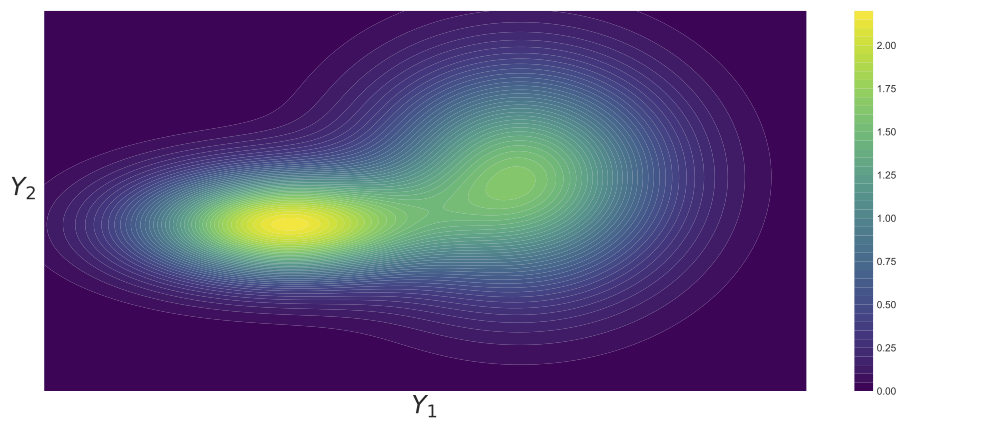
\includegraphics[width=.95\textwidth]{figures/chapter02/energy-landscape.pdf}
    \caption{}
    \label{fig:Energy}
  \end{subfigure}
  \begin{subfigure}{.48\textwidth}
    \centering
    \includegraphics[width=.95\textwidth]{figures/chapter02/pdf-landscape.pdf}
    \caption{}
    \label{fig:pdf}
  \end{subfigure}
  \caption{The energy landscape of a 2D bi-modal distribution (\textbf{a}) and the corresponding probability density function (\textbf{b}).}
\end{figure*}
We have already encountered the term energy when discussing Gibbs distribution as parameterisation of Markov networks. An energy-based model (EBMs)  defines a parametric Gibbs distribution as
\begin{align}
  P_{\bm{\theta}}(Y=\bm{y}) = \frac{1}{Z(\bm{\theta})} e^{-E_{\bm{\theta}}(\bm{y})},
\end{align}
where $E_{\bm{\theta}}(\cdot): \mathcal{Y}\rightarrow \mathbb{R}$ is dubbed energy function and $Z(\bm{\theta})$ is called the partition function. For example, the \Cref{fig:Energy} shows the energy function of a 2D distribution with two modes, the integral over the suppose is not equal to $1$ but the energy is proportional to .

EBMs allow us to parameterise probability distributions with free-form neural networks taking values in $\mathbb{R}$. This is particularly appealing as it unlocks the use of any architecture in contrast to other deep probabilistic models. These models have the precious ability to combine the flexibility of neural networks with the architectural inductive bias critical to the greatest successes of deep learning. However, there is a price to pay in exchange. These models do not grant access to the likelihood function, and we must ellaborate innovative strategies to approximate MLE.

We can directly compute the partition function in the discrete case. We can easily access the model's likelihood function and learn the model with MLE. In the continuous setting - $\mathcal{Y} \triangleq \mathbb{R}^d$, approximating the likelihood is the main challenge for learning EBMs. We review three strategies that enable us to learn continuous EBMs.

The most natural strategy is to approximate the normalising factor with Monte Carlo estimation. However, this requires to sample from the energy-based model, which is not immediate either. A solution is to resort to sampling strategies that work with unnormalised distributions, such as MCMC techniques.

\paragraph{Contrastive learning.}
Strategies that avoid resorting to sampling exist. In particular, \citet{gutmann2012noise} proposed using contrastive learning to train the EBM and estimate the normalising constant jointly. The intuition is that if the energy function models correctly the training distribution, it should enable discriminating between noise and samples from the distribution. Indeed, let us consider a balanced binary classification problem where samples from class $0$ follow a known noise distribution $P_n$, and class $1$ is the training set. As long as the supports of the noise and the training distributions match, the Bayes optimal classifier is a function of the log ratio between the two densities. Then learning corresponds to minimising a cross-entropy loss of a classifier expressed as a function of the EBM. This strategy is sensitive to the distribution of the noise. In particular, it often leads to inaccurate estimation of the energy landscape in low-density regions of the noise distribution. We can roughly interpret generative adversarial networks (GANs) as some contrastive learning of an EBM where the noise distribution is the generator and evolves along with training. The discriminator implicitly defines the energy function. Similarly, \citet{grathwohl2019your} noticed that any classifier could be seen as an EBM. It is interesting to note that contrastive learning could be particularly well suited for transferring an explicit generative model to a new dataset with similar support.

\paragraph{Score matching.}
Score matching \citep{hyvarinen2005estimation} fixes the innacuracy of contrastive learning in low density regions of the noise distrubution. This training strategy notices that the score function, the gradient of the log-likelihood with respect to the data, is independent from the partition function. Thus learning a good energy function can be achieved by minimizing the distance between the model score function $-\nabla_Y E_{\bm{\theta}}(Y=\cdot): \mathbb{R}^d \rightarrow \mathbb{R}^d$, and the data score function $\bm{s}(\cdot)\triangleq \nabla_Y \log P(Y=\cdot): \mathbb{R}^d \rightarrow \mathbb{R}^d$. Formally this leads to the following optimization problem
\begin{align}
  \bm{\theta}^{\star} = \argmin_{\bm{\theta}} \int_{\bm{y} \in \mathbb{R}^d} P(Y=\bm{y}) \lVert \bm{s}(\bm{y}) + \nabla_Y E_{\bm{\theta}}(\bm{y})\rVert^2 \text{d}\bm{y}. \label{eq:score_matching}
\end{align}
This formulation is still difficult to optimise as it would require accessing the data's score function, which is what we are implicitly trying to estimate by learning the energy function. However, under weak regularity conditions, we can express the objective function in \Cref{eq:score_matching} as
\begin{align}
  J(\bm{\theta}) = \int_{\bm{y} \in \mathbb{R}^d} P(Y=\bm{y}) \sum_{i=1}^d \frac{-\partial \nabla_Y E_{\bm{\theta}}[i]}{\partial y_i } + \frac{1}{2} (\nabla_Y E_{\bm{\theta}[i]})^2 + C,
\end{align}
where $\nabla_Y E_{\bm{\theta}}[i] = \frac{\partial E_{\bm{\theta}}}{\partial y_i}$ is the partial derivative of the energy function with respect to the $\text{i}^{\text{th}}$ component of the input vector $\bm y$. The constant $C$ is independent from the parameters $\bm \theta$ and the objective function directly translate into a loss function if we use neural networks to model the energy function. We note that score matching does not perform maximum likelihood estimation of the parameters. While MLE corresponds to searching for the best models with the KL divergence, score matching has a correspondance with the Fisher divergence \citep{lyu2012interpretation}.

It is interesting to note that back in 2010, \citet{vincent2011connection} suggested to use score matching to learn denoising models - models that represents the conditional distribution $P(Y\mid \tilde Y)$ of a clean random variable $Y$ given a noisy version $\tilde{Y} = Y + n$ perturbed by some noise $n$ (e.g. a white Gaussian noise). This idea naturally brings us to diffusion models that have recently become state-of-the-art deep generative models for image synthesis.
\subsection{Diffusion models}
Diffusion models encompass deep generative models that are all connected by the idea of corrupting structured data into noise and learning a model that reverses the corruption process. We distinguish two sub-classes of diffusion models: 1) Continuous-time models \citep{song_generative_2019, song2020score} that formalise the diffusion and generative process as stochastic differential equations and learn the model with denoising score-matching; 2) Discrete-time models dubbed \textit{denoising diffusion probabilistic models}~\citep[DDPM][]{sohl-dickstein_deep_2015, ho_denoising_2020} that fix the number of corruption steps as a hyperparameter of the model and use variational inference to derive a bound on the model's likelihood. We first provide a thorough description of discrete-time models and then discuss intuitively continuous-time. We encourage the reader interested in continuous-time models to look at the following papers for more information: \citep{song_generative_2019, song2020score, song2021maximum, dockhorn2021score}.

\paragraph{Discrete-time diffusion.}
\begin{figure*}
    \centering
    \begin{subfigure}{.75\textwidth}
  \centering
  \begin{tikzpicture}[
    node distance=.1cm and 1.cm,
    mynode/.style={draw, circle, text width=.7cm, align=center},
    simple/.style={align=center},
    simplebis/.style={align=center, text width=1.7cm},
]
\node[mynode] (b) at (0, 0) {$Y_{T}$};
\node[simple, right=of b] (c) {$\dots$};
\node[simple, right=of b] (c) {$\dots$};
\node[mynode, right=of c] (d) {$Y_{t}$};
\node[mynode, right=of d] (e) {$Y_{t-1}$};
\node[simple, right=of e] (f) {$\dots$};
\node[mynode, right=of f] (g) {$Y$};

\node[simplebis, above=of b]  (Y_T) {$\mathcal{N}(\mathbf{0}, I)$};
\node[simple, above=of e]  (Z) {$P_{\bm{\theta}}(Y_{t-1}|Y_{t})$};
\node[simple, above=of g]  (Z) {$\approx P(Y)$};


\path (b) edge[-latex] (c);
\path (c) edge[-latex] (d);
\path (d) edge[-latex] (e);
\path (e) edge[-latex] (f);
\path (f) edge[-latex] (g);

\end{tikzpicture}
  \caption{}
  \label{}
\end{subfigure}

\vspace{2em}

\begin{subfigure}{.75\textwidth}
  \centering
  \begin{tikzpicture}[
    node distance=.1cm and 1.cm,
    mynode/.style={draw, circle, text width=.7cm, align=center},
    simple/.style={align=center},
    simplebis/.style={align=center, text width=1.7cm},
]
\node[mynode] (b)  at (0, 0) {$Y_{T}$};
\node[simple, right=of b] (c) {$\dots$};
\node[mynode, right=of c] (d) {$Y_{t}$};
\node[mynode, right=of d] (e) {$Y_{t-1}$};
\node[simple, right=of e] (f) {$\dots$};
\node[mynode, right=of f] (g) {$Y$};


\node[simple, below=of d]  (Y_T) {$Q(Y_{t}|Y_{t-1})$};
\node[simple, below=of g]  (Z) {$P(Y)$};
\node[simplebis, below=of b]  (Z) {$\approx \mathcal{N}(\mathbf{0}, I)$};

\path (b) edge[latex-] (c);
\path (c) edge[latex-] (d);
\path (d) edge[latex-] (e);
\path (e) edge[latex-] (f);
\path (f) edge[latex-] (g);

\end{tikzpicture}
\caption{}
\label{}
\end{subfigure}
\caption{The description of a discrete-time diffusion with Bayesian networks, more precisely Markov chains. \textbf{(a)} The reverse (generative) process samples an initial state from a normal distribution and generates observations $Y$ by transiting between states with the learned conditional distribution $P_{\bm{\theta}}(Y_{t-1}|Y_{t})$. \textbf{(b)} The diffusion process progressively corrupts observations from the dataset $Y \sim P(Y)$ with a prescribed corruption kernel $Q(Y_{t}|Y_{t-1})$ that eventually converge to noise.}
\label{fig:DDPM}
\end{figure*}
Inspired by non-equilibrium statistical physics, \citet{sohl-dickstein_deep_2015} originally introduced DDPMs. \citet{ho_denoising_2020}  demonstrated only more recently how to train these models for image synthesis and achieved results close to the state-of-the-art on this task. DDPMs formulate generative modelling as the reverse operation of diffusion, a physical process which progressively destroys information. These processes takes the form of Markov chains as depicted in \Cref{fig:DDPM}.

Formally, the reverse process is a latent variable model of the form
$$P_{\bm{\theta}}(Y=\mathbf{y}) := \int P_{\bm{\theta}}(\mathbf{y}_{0:T}) d\mathbf{y}_{1:T},$$
where $\mathbf{y}_0:=\mathbf{y} \in \mathbb{R}^d$ denotes the observations and $\mathbf{y}_1, \dots, \mathbf{y}_T$ denote latent variables of the same dimensionality as $\mathbf{y}$. The joint distribution $P_{\bm{\theta}}(\mathbf{y}_{0:T})$ is modelled as a first order Markov chain with Gaussian transitions, that is
\begin{align}
    &P_{\bm{\theta}}(\mathbf{y}_{0:T}) := P_{\bm{\theta}}(\mathbf{y}_{T}) \prod^T_{t=1} P_{\bm{\theta}}(\mathbf{y}_{t-1}|\mathbf{y}_{t}),\\
    & \text{where } P_{\bm{\theta}}(\mathbf{y}_{T}) := \mathcal{N}(\mathbf{0}, \text{I}) \quad \text{ and } \quad P_{\bm{\theta}}(\mathbf{y}_{t-1}|\mathbf{y}_{t}) := \mathcal{N}(\mathbf{\mu_\psi}(\mathbf{y}_t, t), \sigma_t^2 \text{I}).
\end{align}
We want to estimate the parameters of the generative (reverse) process with maximum likelihood estimation. However, we do not have access to the likelihood function $P_{\bm{\theta}}(Y=\mathbf{y})$ explicitly but only to the joint distribution between the observation and the latent variables $P_{\bm{\theta}}(\mathbf{y}_{0:T})$. This is exactly the setting that motivated us to discuss and derive the $\operatorname{ELBO}$ in \Cref{eq:elbo}.
Here, the approximate posterior $Q(\mathbf{y}_{1:T}|\mathbf{y}_0)$ is a diffusion process that is also a first order Markov chain with Gaussian transitions,
\begin{align}
    &Q(\mathbf{y}_{1:T}|\mathbf{y}_0) := \prod^T_{t=1} Q(\mathbf{y}_{t}|\mathbf{y}_{t-1}),\\
    &Q(\mathbf{y}_{t}|\mathbf{y}_{t-1}) := \mathcal{N}(\sqrt{1-\beta_t} \mathbf{y}_{t-1}, \beta_t \text{I}),
\end{align}
where $\beta_1, \hdots, \beta_T$ are the variance schedule that is either fixed as training hyper-parameters or learned.
The $\operatorname{ELBO}$ is then given by
\begin{align}
    \operatorname{ELBO} := \mathbb{E}_Q\left[ \log \frac{P_{\bm{\theta}}(\mathbf{y_{0:T}})}{Q(\mathbf{y_{1:T}}|\mathbf{x_0})} \right] \leq \log P_{\bm{\theta}}(\mathbf{y}_0). \label{eq:ELBO_DDPM}
\end{align}

Provided that the variance schedule $\beta_t$ is small and that the number of timesteps $T$ is large enough, the Gaussian assumptions on the generative process $P_{\bm{\theta}}$ are reasonable. \citet{ho_denoising_2020} take advantage of the Gaussian transitions to express the $\operatorname{ELBO}$ as
\begin{align}
        \mathbb{E}_Q \biggl[& \mathbb{KL}\left[Q(\mathbf{y}_T|\mathbf{x}_0)\Vert p(\mathbf{y}_T)\right] - \log P_{\bm{\theta}}(\mathbf{y}_0|\mathbf{y}_1) + \sum_{t=2}^T \mathbb{KL}\left[q(\mathbf{y}_{t-1}|\mathbf{y}_t, \mathbf{y}_0)\Vert P_{\bm{\theta}}(\mathbf{y}_{t-1}|\mathbf{y}_t)\right]
     \biggr]. \label{eq:simple_DDPM_ELBO}
\end{align}
The inner sum in \Cref{eq:simple_DDPM_ELBO} is made of comparisons between the Gaussian generative transitions $P_{\bm{\theta}}(\mathbf{y}_{t-1}|\mathbf{y}_t)$ and the conditional forward posterior $Q(\mathbf{y}_{t-1}|\mathbf{y}_t, \mathbf{y}_0)$ which can also be expressed in closed form as Gaussians $\mathcal{N}(\tilde{\mu}_t(\mathbf{y}_0, \mathbf{y}_t), \tilde{\beta}_t \text{I})$, where $\tilde{\mu}_t$ and $\tilde{\beta}_t$ depends on the variance schedule. The KL can thus be calculated with closed form expressions which reduces the variance of the final expression.
In addition, \citet{ho_denoising_2020} empirically demonstrate that it is sufficient to take optimisation steps on uniformly sampled terms of the sum instead of computing it completely. The final objective resembles denoising score matching over multiple noise levels \citep{vincent2011connection}. These observations, combined with additional simplifications, lead to a simplified loss
\begin{align}
    L_\text{DDPM}(\mathbf{y}_0; \bm{\theta}) := \mathbb{E}_{t, \mathbf{y}_0, \mathbf{y}_t}\left[ \frac{1}{2\sigma^2_t}\lVert \mathbf{\mu}_{\bm{\theta}}(\mathbf{y}_t, t) - \tilde{\mu}_t(\mathbf{y}_0, \mathbf{y}_t)  \rVert^2\right],
\end{align}
where $\tilde{\mu}_t(\mathbf{y}_0, \mathbf{y}_t)$ is the mean of $Q(\mathbf{y}_{t-1}|\mathbf{y}_{0}, \mathbf{y}_{t})$, the forward diffusion posterior conditioned on the observation $\mathbf{y}_{0}$. We refer the reader to \citet{ho_denoising_2020} for the detailed derivation of the simplified loss function.

\paragraph{Continuous-time diffusion.}
Denoising score matching and DDPM rest on perturbing data at multiple noise scales. Continuous-time diffusion generalises this idea to an infinite number of noise scales corresponding to formulating the forward and reverse processes as stochastic differential equations (SDE). \citet{song2020score} formally describe the diffusion process as the solution to an It{\^o} SDE:
\begin{align}
  \text{d}\bm{y} = \bm{f}(\bm{y}, t) \text{d}t + g(t) \text{d}\bm{w}, \label{eq:continuous_diffusion}
\end{align}
where $\bm{w}$ is the standard Wiener process (a.k.a., Brownian motion), $\bm{f}(\cdot, t): \mathbb{R}^d \rightarrow \mathbb{R}^d$ is a vector-valued function called the drift coefficient of $\bm{y}(t)$, and $g(\cdot): \mathbb{R} \rightarrow \mathbb{R}$ is a scalar function known as
the diffusion coefficient of $\bm{y}(t)$.

In this formulation, $\bm{y}(\cdot): \mathbb{R} \rightarrow \mathbb{R}^d$ becomes a function of time where initial states $\bm{y}(0)$ are provided by the training samples. We design the drift and diffusion coefficients to enforce a known noise distribution $p_T$ (e.g., $p_T = \mathcal{N}(\bm 0, I)$) after running the SDE from $t=0$ to $t=T$. We can then generate artificial samples from $P_0 = P(Y)$ by sampling an initial state $\bm{y}_T \sim p_T$ and running the reverse SDE defined by \citet{anderson1982reverse} as
\begin{align}
  \text{d}\bm{y} = \left[ \bm{f}(\bm{y}, t) \text{d}t - g(t)^2 \nabla_Y \log P_t(Y=\bm{y}) \right] \text{d}t + g(t) \text{d}\bm{w},\label{eq:continuous_reverse_diffusion}
\end{align}
where the Wiener process and time flow from $t=T$ to $t=0$. The reverse process closely resembles stochastic Langevin dynamics with infinitesimal steps.

The score functions $\nabla_Y \log P_t(Y=\bm{y})$ are indexed by time $t$ and parameterized by a neural network $\bm{s}_{\bm{\theta}}(\cdot, t) : \mathbb{R}^d \rightarrow \mathbb{R}^d$ that takes both the state $\bm{y}(t)$ and the time $t$. We train the neural networks with score matching at all noise scales. Formally, the learning problem is
\begin{align}
  \bm{\theta}^\star = \argmin_{\bm{\theta}} \mathbb{E}_t\Bigg[ \mathbb{E}_{\bm{y}(0)} \mathbb{E}_{\bm{y}(t)\mid \bm{y}(0)}\left[ \lVert \bm{s}_{\bm{\theta}}(\bm{y}(t), t) - \nabla_{Y_t} \log P_{0:t}\Big(\bm{y}(t) \mid \bm{y}(0)\Big) \rVert^2 \right] \Bigg]. \label{eq:continuous_diffusion_objective}
\end{align}
For adequatte drift and diffusion coefficients, the diffusion kernel $P_{0:t}\Big(\bm{y}(t) \mid \bm{y}(0)\Big)$ is easy to sample from and can be evaluated in closed-form. And we can use Monte Carlo estimations of the objective function in \Cref{eq:continuous_diffusion_objective} to train a neural network with stochastic gradient descent. We can resort to sliced score matching \citep{song2020sliced} to optimize $\bm{s}_{\bm{\theta }}$ from samples of the forward process when the diffusion kernel cannot be evaluated directly.

There exists a duality between SDEs and ordinary differential equations (ODE) that allows us to transform one into the other while maintaining the same marginal distribution over the states. The ODE corresponding to \Cref{eq:continuous_reverse_diffusion} is
\begin{align}
  \text{d}\bm{y} = \left[ \bm{f}(\bm{y}, t) - \frac{1}{2}g(t)^2 \nabla_Y \log P_t(Y=\bm{y}) \right] \text{d}t.
\end{align}
Provided the approximation $\bm{s}_{\bm{\theta}}$ and an initial random state $\bm{y}_T \sim P_T$ we can then use an ODE solver to generate samples.

This duality is very important as it provides a direct way of evaluating the model's likelihood via the instantaneous change of variables. This theorem states that the change in log probability of a continuous random variables $\bm{y}(t) \sim P(\bm{y}(t))$ transformed by an ODE $\frac{\text{d}\bm{y}}{\text{d}t} = \bm{h}(\bm{y}(t), t)$, where $\bm{h}$ is uniformly Lisphitz, follows a differential equation
\begin{align}
  \frac{\partial \log P(\bm{y}(t))}{\partial t} = -\operatorname{tr}(\frac{d\bm{h}}{\text{d}\bm{y}(t)}), \label{eq:NODE_NF}
\end{align}
where $\operatorname{tr}(\frac{d\bm{h}}{\text{d}\bm{y}(t)})$ is the trace of the Jacobian of $\bm{h}$. This draws a direct connection between diffusion models and normalizing flows that constitute the next class of deep probabilistic models we are going to discuss.

\subsection{Normalizing flows}
A Normalizing Flow~\citep[NF, ][]{rezende2015variational} is defined as a sequence of invertible transformations $\mathbf{u}_i : \mathbb{R}^d \to \mathbb{R}^d$  ($i=1, ..., k$) composed together to create an expressive invertible mapping $\mathbf{u} = \mathbf{u}_1 \circ \dots \circ \mathbf{u}_k : \mathbb{R}^d \to \mathbb{R}^d$. This mapping can be used to perform density estimation, using $\mathbf{u}(\cdot ;\mathbf{\theta}): \mathbb{R}^d \rightarrow \mathbb{R}^d$ to map a sample $\mathbf{y} \in \mathbb{R}^d$ onto a latent vector $\mathbf{z} \in \mathbb{R}^d$ equipped with a prescribed density $P_{\mathbf{z}}(\mathbf{z})$ such as an isotropic Normal. The transformation $\mathbf{u}$ implicitly defines a density $p(\mathbf{x}; \mathbf{\theta})$ as given by the change of variables formula,
\begin{equation}
    P(\mathbf{y}; \mathbf{\theta}) = P_Z(\mathbf{u}(\mathbf{y};\mathbf{\theta})) \left| \det  J_{\mathbf{u}(\mathbf{y};\mathbf{\theta})} \right|, \label{eq:NF_DE}
\end{equation}
where $J_{\mathbf{u}(\mathbf{y};\mathbf{\theta})}$ is the Jacobian of $\mathbf{u}(\mathbf{y};\mathbf{\theta})$ with respect to $\mathbf x$.
The resulting model is trained by maximising the likelihood of the data $\{\mathbf{y}^1, ..., \mathbf{y}^N\}$.

It is common for normalizing flows to stack the same parametric function $\mathbf{u}_i$ (with different parameters values) and to reverse variables ordering after each transformation. For this reason, we will focus on presenting a popular strategy to build one of these repeated transformations, which we further refer to as $\mathbf{g}: \mathbb{R}^d\rightarrow \mathbb{R}^d$.

In general the steps $\mathbf{g}$ can take any form as long as they define a bijective map. Many neural architectures of normalizing flows can be mathematically described as
\begin{align}
    \mathbf{g}(\mathbf{y}) = \begin{bmatrix}
g^1(y_{1}; \mathbf{c}^1(\mathbf{y}))  & \hdots & g^d(y_{d}; \mathbf{c}^d(\mathbf{y}))
\end{bmatrix}^T,\label{eq:gnf}
\end{align}
where the $\mathbf{c}^i$ are the \textbf{conditioners} which role is to constrain the structure of the Jacobian of $\mathbf{g}$ into triangularizable matrices. The functions $g^i$, called \textbf{normalizers}, partially parameterized by their conditioner, must be invertible with respect to their input variable $y_i$. For such architectures, the determinant of the Jacobian reduces to the product of the partial derivatives $\frac{\partial g^i}{\partial y_i}$, which is sign-constant. This implies that the determinant of the Jacobian never cancels out and convinces us that $\mathbf{g}$ is bijective.

The conditioners impose an autoregressive structure or, more generally, any structure representing a directed acyclic graph. In \Cref{ch:04} and \Cref{ch:06}, we show why this is true and draw a clear relationship between normalizing flows and Bayesian networks. The normalizer $g^i$ can be any function as long as it is a monotonic function of its main input $y_i$. In terms of neural networks, an affine normalizer $g: \mathbb{R} \times \mathbb{R}^2 \rightarrow \mathbb{R}$ can be expressed as
$g(x;m, s) = x\exp(s) + m$, where $m \in \mathbb{R}$ and $s \in \mathbb{R}$ are computed by the conditioner. There also exist methods to parameterize monotonic normalizers \citep{huang_neural_2018, de_cao_block_2020, durkan_neural_2019, jaini_sum--squares_2019} with neural networks and one contribution of this thesis is to introduce one of them called Unconstrained Monotonic Neural Networks~\citep[UMNNs, ][]{wehenkel_unconstrained_2019} in \Cref{ch:05}.

We have described discrete normalising flows for which $k$ is a finite number. There also exist continuous normalizing flows that correspond to infinitesimal transformations defined by an ODE $\frac{\text{d} \bm{y} }{\text{d}t} = \bm{h}(\bm{y}(t), t)$ as mentioned at the end of the discussion on diffusion models. Continuous NFs were first introduced in the seminal work on neural ordinary equations by \citet[NODE,][]{chen_neural_2018}. Soon after, \citet{grathwohl_ffjord_2018} proposed to use the Hutchinson trace estimator in \Cref{eq:NODE_NF} to reduce the computation cost of continuous NFs. As previously mentioned, continuous NFs can be parameterised by any Lipshitz continuous function and are thus easy to parameterise with neural networks. This is not as simple for discrete NFs, which is why the rest of this discussion is only about discrete flows. This discussion aims to provide an overview of the main characteristics of NFs and some existing parameterisation. \citet{papamakarios_normalizing_2019, kobyzev_normalizing_2020} will provide additional details to the greedy reader.

Remarkably, NFs are the only deep probabilistic model that explicitly provides access to the likelihood function, hence to the learned density. In contrast to other deep probabilistic models that require tricks to formulate a tractable optimisation problem, the learning algorithm of NFs is straightforward. It is just the gradient descent of the negative log-likelihood. Explicit models are also particularly interesting for parameterising the approximate posterior in VI~\citep{rezende2015variational} and have played an essential role in many simulation-based inference algorithms as well \citep{papamakarios_sequential_2019, greenberg_automatic_2019}.

The tractability of the likelihood function has a price. Discrete NFs require strongly constraining the architecture used to parameterise the bijective transformations. This often leads to poor inductive bias and reduces these models' efficiency for some data modalities such as images. For continuous models, the principal cost is the potential complexity of solving the associated neural ODE and the difficulty of optimising NODE models. In general, the most fundamental issue of NFs is to enforce a latent space that has the same dimensionality as the data whereas it is often more reasonable to assume these data lie on a lower-dimensional manifold. People have worked at solving this issue, e.g., \citet{brehmer2020flows} introduced $\mathcal{M}\text{-flow}$ that learns a manifold and a density on it jointly; however these methods either requires a prescribed manifold, or they resort to adversarial optimization which cut down the simple training loop of classical NFs.

A simpler solution is to formulate the generative process as a stochastic mapping between low dimensional latent variables to observations instead and use NFs to model conditional distributions. These models are called variational auto-encoders and are covered below.

\subsection{Variational auto-encoders}
\begin{figure*}
    \centering
    \begin{subfigure}{.45\textwidth}
  \centering
  \begin{tikzpicture}[
    node distance=.1cm and 1.cm,
    mynode/.style={draw, circle, text width=.4cm, align=center},
  simple/.style={text width=2cm,align=center}
]
\node[mynode] (x1) {$Y$};
\node[mynode, left=of x1] (z1) {$Z$};
\node[simple, above=of x1]  (Y_Z) {$P_{\mathbf{\theta}}(Y\mid Z)$};
\node[simple, above=of z1]  (Z) {$P(Z)$};

\path (z1) edge[-latex] (x1);

\end{tikzpicture}
  \caption{}
  \label{}
\end{subfigure}
\begin{subfigure}{.45\textwidth}
\centering
\begin{tikzpicture}[
node distance=.1cm and 1.cm,
mynode/.style={draw, circle, text width=.4cm, align=center},
simple/.style={text width=2cm,align=center}
]
\node[mynode] (x1) {$Y$};
\node[mynode, left=of x1] (z1) {$Z$};
\node[simple, above=of x1]  (Y_Z) {$P(Y)$};
\node[simple, above=of z1]  (Z) {$Q_{\bm{\psi}}(Z\mid Y)$};

\path (x1) edge[-latex] (z1);

\end{tikzpicture}
\caption{}
\label{}
\end{subfigure}
\caption{The description of a variational auto-encoder with Bayesian networks. \textbf{(a)} The decoding process samples the latent variables from $P(Z)$ and generates observations $Y$ by sampling conditionaly from $P_{\mathbf{\theta}}(Y\mid Z)$. \textbf{(b)} The encoding process takes an observation from the dataset $Y \sim P(Y)$ and computes the approximate posterior $Q_{\bm \psi}(Z\mid Y)$ corresponding to the model in \textbf{(a)}.}
\end{figure*}

We have already discussed some generative models based on latent variables with diffusion models. The main difference here is to not assume a prescribed mapping from the observations $Y$ to the latent $Z$. Instead a variational auto-encoder~\citep[VAE, ][]{kingma_auto-encoding_2013} trains jointly an encoder network that models the posterior distribution $Q_{\bm \psi}(Z\mid Y) \approx P(Z\mid Y) $ and a decoder network that parameterizes the stochastic mapping $P_{\bm \theta}(Y\mid Z)$ from latent variables to observations. This allows us to embed good inductive bias in the decoder that generates observations from latent variables. A good example is the NVAE~\citep{vahdat_nvae_2020} that formulates this mapping hierarchically for images, using different latent variables to describe the high-level and low-level structure of the image.

Formally, we want to learn a generative model of an unknown distribution $P(Y)$ given a dataset $\mathcal{D} \triangleq \{\mathbf{y}^i\}^N_{i=1}$ of $N$ i.i.d observations $\mathbf{y}^i \sim P(Y)$ sampled from this unknown distribution.
The original VAE postulates a two-step generative process in which some unobserved variables $\mathbf{z} \in \mathbb{R}^h$ are first sampled from a prior distribution $P(Z)$ and then observations $\mathbf{y}$ are generated from a conditional distribution $P_{\mathbf{\theta}}(Y\mid Z=\mathbf{z})$. The generative process can be expressed mathematically as
\begin{align}
     \mathbf{z} \sim P(Z) \quad \text{and} \quad \mathbf{y} \sim P_{\mathbf{\theta}}(Y\mid Z=\mathbf{z}).
\end{align}
The prior $P(Z)$ is often an isotropic Gaussian while the likelihood $P_{\mathbf{\theta}}(X\mid Z=\mathbf{z})$ is parameterised with a neural network. The likelihood model decodes latent variables into observations and is thus usually referred to as the decoder in the literature. In its original formulation, the likelihood is parameterized with a multivariate Gaussian $\mathcal{N}\bigg(\mathbf{\mu_\theta}(\mathbf{z}), \diag\big(\sigma_\theta^2(\mathbf{z})\big)\bigg)$ when the domain $\mathcal{Y}$ is continuous, and a categorical distribution when it is discrete.

Training aims to find the parameters $\mathbf{\theta}$ of the decoder that maximize the sum of the marginal likelihoods of individual points, the MLE which optimises $$\log P_{\mathbf{\theta}}(Y)= \sum_{\mathbf{y}\in \mathcal{D}}\log \int P_{\mathbf{\theta}}(\mathbf{y}\mid \mathbf{z}) P(\mathbf{z}) \text{d}\mathbf{z}.$$

These integrals are intractable but we rely on variational inference again to approximate the MLE objective. The introduction of an encoder network that approximates the posterior distribution $Q_{\bm \psi}(Z\mid Y)$ allows maximizing the associated evidence lower bound
\begin{align}
    \operatorname{ELBO}(\bm{y}; \mathbf{\theta}, \mathbf{\psi})&:=\mathbb{E}_Q\left[\log \frac{P_{\mathbf{\theta}} (\mathbf{y}\mid \mathbf{z}) P(\mathbf{z})}{Q_\psi(\mathbf{z}\mid \mathbf{y})} \right]\label{eq:ELBO_VAE}\\
    &=\log P_{\mathbf{\theta}}(\mathbf{y}) - \mathbb{KL}\left[Q_{\bm \psi}(Z\mid \mathbf{y})\Vert P_{\mathbf{\theta}} (Z\mid \mathbf{y})\right]\\
    &\leq \log P_{\mathbf{\theta}}(\mathbf{x}).
\end{align}

The $\operatorname{ELBO}$ becomes tighter as the approximate posterior $Q_{\bm \psi}(\mathbf{z}|\mathbf{y})$ gets closer to the true posterior.
Learning the generative model is finally performed by jointly optimising the parameters $\mathbf{\theta}$ of the decoder and ${\bm \psi}$ of the approximate posterior via stochastic gradient ascent.
In the original VAE, the encoder models the approximate posterior as a conditional multivariate Gaussian distribution $\mathcal{N}(\mu_{\bm \psi}(\mathbf{y}), \diag(\sigma_{\bm\psi}^2(\mathbf{y})))$.

In practice, the good optimisation of VAEs depends on the ability of the encoder $Q_{\bm \psi}(Z|Y)$ to approximate the posterior well at all possible observations $Y$. This also implies that marginalizing out $Y$ from the encoder - i.e. $Q(Z) \triangleq \frac{1}{N}\sum_{\bm{y}_i \in \mathcal{D}} Q_{\bm \psi}(Z|Y)$ - should closely match the prior distribution $P(Z)$ which is often difficult. A strategy is to make both the posterior and prior distribution generic by parameterising them with normalizing flows.
\subsection{Discussion}
As we have seen the separation between two classes of models is sometimes blurry. NFs and autoregressive models have more in common than differences. Similarly, the only difference between a classical VAE and a diffusion model is on the parameterization of the approximate posterior distribution. Moreover diffusion models ends up achieving the exact same goal as a NF, it maps a noise distribution to the data distribution with an invertible transformation. Energy based models are slighlty more distinct in contrast but most of the algorithms relevant to unnormalized models end up being also interesting for other models such as continuous diffusion models.

In this background, we let aside some aspects of deep generative models because we do not believe these are necessary to aprehend the rest of this thesis. In particular, we avoid providing details about the neural architectures used in practice although this is decisive for achieving good performance with deep probablistic models. These choices are usually motivated by experience and depends on the type of data. New architectures leading to better performance in discriminative tasks often leads to progress in the corresponding unsupservised modelling tasks. In addition, there also exist deep architectures specialized for to sub-classes of deep probabilistic models such as hierarchical VAEs \citep{vahdat_nvae_2020}, causal convolutions \citep{van_den_oord_wavenet_2016}, etc... Furthermore, years of research in deep probablistic models has lead to many tricks that can improve the performance of these models in different contexts.
% - Say there exist many variations of these algorithms (e.g. hierarchical vae, implicit diffuion, ...).

% \section{The multiple definitions of hybrid modelling}
% - hybrid modelling can be combining discrete and continuous variables. This is not something we consider in  this thesis.
% - We instead consider hybrid learning as fitting a simple class of models, e.g. a parametetric relationship between some interpretable latent variables and the observations, together with a deep probablistic models that can correct for the misspecification of small models.

\section{Chalenges and opportunities}
We have now presented the main deep probabilistic models (DPMs). All these models offer a different balance between simplicity, tractability and expressivity. Some models, such as diffusion and energy-based models, define the probabilistic model implicitly and even involve sampling algorithms to express the modelled distribution. For others, such as NFs and autoregressive models, the distribution is modelled explicitly - we can access the model's likelihood. Sampling these models is not always computationally efficient but is a deterministic procedure that does not depend on any hyperparameters in contrast to diffusion and energy-based models. Finally, VAEs offer a nice balance between expressivity and tractability. Although the model's likelihood is only approximated via the ELBO, these models are usually easy to sample.

We have also introduced graphical models closer to classical modelling strategies than DPMs. Indeed, the topology, often prescribed, defines a set of strong assumptions on the modelled phenomenon. The learning task mostly amounts to fitting conditional distributions. This is close to classical modelling, where we try to fit together already existing models that are assumed faithful to sub-components of the modelled phenomenon. In contrast, deep models mainly rely on the inductive bias - soft constraints induced by the neural networks' architecture and training algorithm.

 This thesis aims to rub out the borders between different classes of models. We argue that obliterating these connections leads to an unnecessary profusion of specialised algorithms and terminologies that are equivalent. This reduces the accessibility of probabilistic modelling, which is yet one of the most fundamental tools of engineers and scientists. In addition, we foresee at least two other motivations for drawing connections between different types of models. First, it provides a new prospect on the concerned models, which has countless positive outcomes as it unlocks the sharing of algorithms, interpretations, pre-trained models, etc... The second motivation is to simplify the compositionality of different classes of models together, which is critical for creating models aligned with prescribed knowledge. Such compositional models may generalise outside the training distributions and require fewer data as they rely on a more substantial inductive bias.


Aligned with this objective, in the first part of the thesis, we discuss and improve the expressivity of VAEs and NFs. In \Cref{ch:03}, we show that modelling the prior of VAEs with diffusion models is beneficial. Then, in \Cref{ch:04}, we draw connections between NFs and Bayesian networks and prove the limitations of existing architectures that we overcome in \Cref{ch:05} with unconstrained monotonic neural networks. In the second part, we explore techniques to embed a more potent form of inductive bias into DPMs. We demonstrate that Bayesian networks and NFs can serve each other's purpose in \Cref{ch:06}. In \Cref{ch:07}, we show that combining deterministic models and VAEs leads to hybrid models that generalise outside the training distributions under appropriate assumptions. Finally, we reflect on this thesis and provide several high-level research directions for pushing further the interplay between different modelling strategies.

%
% Say that:
% - Drawing connections between different classes of model is important as it allows to betteer understand different aspects of the algorithms.
%   This is very important as these models are complex and better understanding allow to make the right design choice.
% - We want to also argue that composisionality of models is very important. This is how modelling was done historically and it has achieved great success. By drawing connection between models we allow this more naturally. But we also want to push that further by combining strong deterministic models with deep probabilistic models.
% -
%
% \textcolor{red}{Add a schematic view of how different models are related to each others and where we made the connections/contributions}
